%%%%%%%%%%%%%%%%%%%%%%%%%%%%%%  IEEEsample.tex
%%%%%%%%%%%%%%%%%%%%%%%%%%%%%%%%%%%%%%%%%
%%%%%%%%%%%%%%%%%%%%%%%    More information: see the header of IEEEtran.sty
%%%%%%%%%%%%%%%%%%%%%%%
%%%%%%%%%%%%%%%%%%%%%%%%%%%%%%%%%%%%%%%%%%%%%%%%%%%%%%%%%%%%%%%%%%%%%%%%%%%%%%%%
%%%%

\documentclass[10pt,twoside,onecolumn]{IEEEtran}
%\documentclass[conference]{IEEEtran}

%%%\IEEEoverridecommandlockouts

\usepackage[ruled,linesnumbered]{algorithm2e}
%%for algorithm2e package, label has to be following caption in the same line!!!
\renewcommand{\algorithmcfname}{ALGORITHM}
\SetAlFnt{\small}
\SetAlCapFnt{\small}
\SetAlCapNameFnt{\small}
\SetAlCapHSkip{0pt}
\IncMargin{-\parindent}

%% \RequirePackage{times}
%% \RequirePackage{algorithmic}
%% \PassOptionsToPackage{boxed}{algorithm}
%% \RequirePackage{algorithm}
%% \RequirePackage{multicol}
%\renewcommand{\algorithmicrequire}{\textbf{Inputs:}}
%\renewcommand{\algorithmicensure}{\textbf{Outputs:}}
%\DeclareMathAlphabet{\mathtsl}{OT1}{ptm}{m}{sl}

%\def\BibTeX{{\rm B\kern-.05em{\sc i\kern-.025em b}\kern-.08em1
%    T\kern-.1667em\lower.7ex\hbox{E}\kern-.125emX}}

%\newtheorem{theorem}{Theorem}
%\newtheorem{lemma}{Lemma}
%\newtheorem{example}{Example}
%\newtheorem{corollary}{Corollary}

\RequirePackage{amssymb, mathptm}
\usepackage{amsbsy}
\usepackage{amsthm}
\usepackage{graphicx}
\usepackage{helvet}
\usepackage{enumerate}
\usepackage{amsmath}
\usepackage{amsfonts}
\usepackage{graphicx}
\usepackage{multirow}
\usepackage{subfig}
\usepackage{comment}
\usepackage{cases}
\usepackage{leqno}
\usepackage{subfigure}

%%indent in algorithm


%\setcounter{page}{1}


% New command for the table notes.
\def\tabnote#1{{\small{#1}}}

% New command for the line spacing.
\newcommand{\ls}[1]
    {\dimen0=\fontdimen6\the\font
     \lineskip=#1\dimen0
     \advance\lineskip.5\fontdimen5\the\font
     \advance\lineskip-\dimen0
     \lineskiplimit=.9\lineskip
     \baselineskip=\lineskip
     \advance\baselineskip\dimen0
     \normallineskip\lineskip
     \normallineskiplimit\lineskiplimit
     \normalbaselineskip\baselineskip
     \ignorespaces
    }
%\renewcommand{\algorithmicrequire}{\textbf{Input:}}
%\renewcommand{\algorithmicensure}{\textbf{Output:}}

\newcommand{\beq}{\begin{equation}}
\newcommand{\eeq}{\end{equation}}
\newcommand{\beqarr}{\begin{eqnarray}}
\newcommand{\eeqarr}{\end{eqnarray}}
%\newcommand{\ov}{\overline}
\newcommand{\ov}{\bar}
\newcommand{\xor}{\bigoplus}
\newcommand{\Fm}{{\mathbb{F}}}
\newcommand{\myfontsize}{\fontsize{7}{9}\selectfont}


%the following is for space before and after align or other equation environment.

%%
\newtheorem{Algorithm}{Algorithm}[section]
\newtheorem{Definition}{Definition}[section]
\newtheorem{Example}{Example}[section]
\newtheorem{Proposition}{Proposition}[section]
\newtheorem{Lemma}{Lemma}[section]
\newtheorem{Theorem}{Theorem}[section]
\newtheorem{Corollary}{Corollary}[section]
\newtheorem{Conjecture}{Conjecture}[section]
\newtheorem{Problem}{Problem}[section]
\newtheorem{Notation}{Notation}[section]
\newtheorem{Setup}{Problem Setup}[section]

%%%

%%set spacing between table columns
\setlength{\tabcolsep}{3pt}

\begin{document}

%\thispagestyle{empty}
%\pagestyle{empty}

%\ls{1.5}


\ls{1.1}

\title{\large{\textsc{Formal Verification of Sequential Galois Field Arithmetic Circuits Using Algebraic Geometry}}}
\author{Xiaojun Sun\\
A Ph.D Thesis Proposal\\
Electrical \& Computer Engineering, University of Utah\\
Fall Semester 2014
}
\maketitle

%\markboth{MS Proposal by Tim Pruss}{}
\newcommand{\Fq}{{\mathbb{F}}_{q}}
\newcommand{\Fkk}{{\mathbb{F}}_{2^k}}
\newcommand{\Ftwo}{{\mathbb{F}}_{2}}
\newcommand{\Fkkx}[1][x]{\ensuremath{\mathbb{F}}_{2^k}[#1]\xspace}
\newcommand{\Grobner}{Gr\"{o}bner\xspace}
\newcommand{\B}{{\mathbb{B}}}
\newcommand{\Z}{{\mathbb{Z}}}
\newcommand{\F}{{\mathcal{F}}}
\newcommand{\G}{{\mathcal{G}}}
%%%

\newcommand{\debug}[1]{\textcolor{gray}{[ #1 ]}}


%%%%%%%%%%%%%%%%%%%% Include your files here %%%%%%%%%%%%%%%%%%%%%
\begin{abstract}
This PhD dissertation proposal addresses the problem of sequential circuit verification at the word-level and is based on concepts derived from algebraic geometry. Analyzing the sequential circuits at word level is an efficient way
of {\it abstraction}, which may  lower the complexity of verification by efficient representation of the state-space. We propose to model the verification properties and the gate-level sequential circuit implementations over Galois fields of the type ${\mathbb{F}}_{2^k}$ by means of polynomial ideals and their canonical representations --- Gr\"obner bases --- at the level of $k$-bit words. Subsequently, techniques from algebraic geometry can be used to reason about the state-space by analyzing varieties of these ideals. 

We propose to apply these techniques to traverse a finite state machine (FSM) for reachability analysis at the word-level, and also to 
implicitly unroll sequential arithmetic circuits to verify their function. Moreover, as unsatisfiable (UNSAT) cores play an important role in modern abstraction-refinement techniques for verification, we propose to investigate a word-level analogue of the UNSAT core problem using the  Gr\"obner basis algorithm. The proposal will not only derive new algorithms and techniques, but will also consider efficient CAD implementations to target sequential equivalence and model checking problems. 
\end{abstract}

\section{Introduction}
\label{sec:intro}

Galois field (GF) arithmetic is part of modern abstract algebra focused on 
computations on modulo-based fields
and finds application in areas such as 
cryptography, error control coding, VLSI testing, etc. In most
hardware applications, fields of the type $\Fkk$ are widely
chosen. Such { binary} GFs are $k$-dimensional extensions
of the base field ${\mathbb{F}}_2$; this allows for the design of
efficient (AND-XOR) arithmetic architectures and algorithms for
hardware design. Due to their deployment in communications and
security-related applications, there is a critical need to {
  formally verify} the correctness of hardware implementations of GF
arithmetic. In most applications, however, the datapath size
(bit-vector operand size) $k$ is too large to use naive enumeration test. Most conventional formal
verification methods are unable to cope with the large size and
complexity of GF circuits. 

GF arithmetic circuits in $\Fkk$ take $k$-bit vectors as inputs and
produce $k$-bit outputs. For example, a GF modulo multiplier computes
$R = A \times B \pmod{ P(x)}$, where: i) $A = a_{s(0)} + a_{s(1)}\alpha +
\dots + a_{s(k-1)} \alpha^{k-1} = \sum _{i=0}^{k-1} a_{s(i)}\alpha^i$,
$B = \sum_{i=0}^{k-1}b_{s(i)} \alpha^{i}$ denote the $k$-bit inputs,
$R = \sum _{i=0} ^{k-1} r_{s(i)} \alpha^i$ is the output, and $a_{s(i)},
b_{s(i)}, r_{s(i)} \in \Ftwo$; ii) $P(x)$ is the given primitive
polynomial used to construct $\Fkk$; and iii) $P(\alpha) = 0$,
i.e, $\alpha$ is the primitive element of the field. In the above, the
elements are represented in { standard basis notation} (denoted by
subscript ``s'' on the bits). As the datapath size $k$ increases,
combinational GF designs become prohibitively large;
%\cite{wu:2002} \cite{acar:1998}; 
sequential GF circuits are therefore desirable. 

Sequential GF circuits operate as follows: $k$-bit input operands are
loaded into $k$-bit state registers (flip-flops), and the circuit is
executed for $k$ clock-cycles; after which the $k$-bit result is
available in the output registers. Data representation and circuit
design for sequential GF circuits is mostly based on { normal basis}
\cite{gao:phd_normal_basis}. Data is represented as $A = a_{n(0)}
\beta + a_{n(1)} \beta^2 + a_{n(2)} \beta^{2^2} + \dots + a_{n(k-1)}
\beta^{2^{k-1}}$, where $\beta \in \Fkk$ is the { normal
  element}, and $\{\beta, \beta^2, \dots, \beta^{2^i}, \dots,
\beta^{2^{k-1}}\}$ forms the normal basis. Standard and normal basis
representations can be derived from each other, i.e, $\beta$ can be
derived from $\alpha$ and vice-versa. It has been shown that
architectures for multiplication and  squaring can be efficiently
designed using normal bases  \cite{agnew1991implementation} 
\cite{RHmulti} \cite{gao:phd_normal_basis} as sequential circuits. 
\footnote{In fact, some (not all) finite fields have an
  { optimal normal basis}, where the combinational logic part of
  the sequential circuit contains a minimum number of 2-input AND/XOR
  gates.}.

\begin{Example}
\label{ex:nb_sq}
For $a, b \in \Fkk, (a+b)^2 = a^2 + b^2$. Applying this rule for
element squaring: 
\begin{align}
B = & (b_0\beta + b_1\beta^2 + b_2\beta^4 + \dots + b_{k-1}\beta^{2^{k-1}}) \nonumber\\
B^2 = &b_0^2\beta^2 + b_1^2\beta^4 + b_2^2\beta^8 + \dots + b_{k-1}^2\beta^{2^k} \nonumber\\
= &b_{k-1}\beta + b_0\beta^2 + b_1\beta^4 + \dots + b_{k-2}\beta^{2^{k-1}} \nonumber
\end{align}
as $\beta^{2^k} = \beta$ due to Fermat's little theorem, and $b_i^2 = b_i$. 
\end{Example}

The above example shows that squaring of elements represented in
normal bases can be implemented simply by a cyclic right-shift
operation. However, multiplication of two elements in normal basis is
still a complicated operation --- and its design and verification is still
challenging. Recent literature has addressed formal equivalence proofs
of { combinational} GF arithmetic circuits \cite{ibm:blueveri}
\cite{lv:tcad2013} \cite{pruss:dac14}. Our research aims to address verification
of sequential GF circuits, which has not been addressed before. 


{\it Problem Statement:} We are given: 
i) the Galois field $\Fkk = \Ftwo[X] \pmod{ P(X)}, P(\alpha) = 0$,
along with the { normal basis representation}, i.e. $\beta$ is also
known; 
ii) a word-level specification polynomial $R = \F(A, B) \pmod{ P(X)}$;
where $A = \sum _{i=0}^{k-1} a_i \beta^{2^{i}}$, $B = \sum
_{i=0}^{k-1} b_i \beta^{2^{i}}$, $R = \sum _{i=0}^{k-1} r_i
\beta^{2^{i}}$, $ a_i, b_i, r_i \in \Ftwo$, and iii) a sequential
circuit ($S$) implementation of the 
polynomial computation. Our objective is to prove or disprove that $S$
is a $k$-cycle implementation of $R$. 

{\it Approach \& Contributions:} The sequential GF arithmetic circuit
can be viewed as a {restricted} Mealy finite state machine (FSM),
as shown in Fig. \ref{fig:sequential}. The FSM contains no
primary inputs or outputs. The operands are loaded into state
registers $A, B$ (as initial states), and after $k$-clock cycles of
operation, the result $R = \F(A, B)$ is stored in the $R$ register. 

\begin{figure}[htb]
\begin{center}
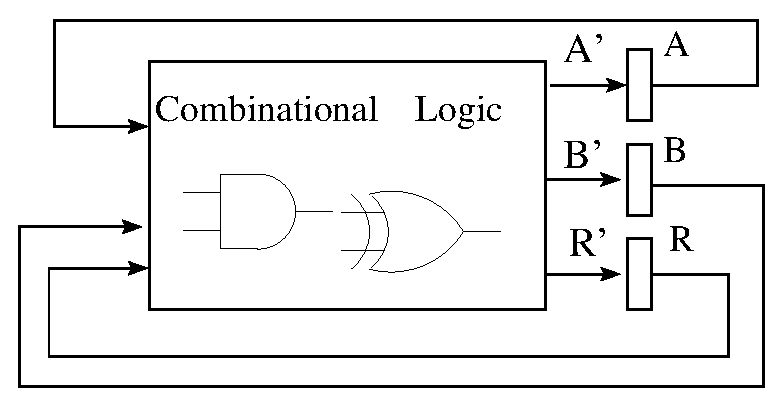
\includegraphics[width=2.8in]{./gf_seq_model.eps}
\end{center}
\caption{\small A typical normal basis GF sequential circuit model. $A =
  (a_0,\dots,a_{k-1})$ and similarly $B, R$ are $k$-bit registers;
  $A', B', R'$ denote next-state inputs.}
\label{fig:sequential}
\end{figure}

% \vspace{-0.2in}
A straightforward approach to verify such a sequential circuit may
consist of unrolling the circuit for $k$ time-frames, and performing a
(combinational) equivalence check between the unrolled machine and the
specification polynomial. Such a technique is grossly inefficient for
large circuits. Therefore, we propose a method that implicitly
(symbolically) represents the unrolled computation, { canonically,
  as a word-level multi-variate polynomial.} We show that the
$k$-cycle polynomial representation can be derived { iteratively}
by performing a sequence of \Grobner basis ($GB$) computations of the
ideal generated by the polynomials corresponding to the circuit. The
approach  requires the use of a specific elimination term order for
the $GB$ computation, based on the circuit's topology. Once the
canonical polynomial is derived, it can be checked against the
specification polynomial for verification.  

Computing \Grobner bases with elimination orders is infeasible for
large circuits. To overcome this complexity, we draw inspiration from
\cite{pruss:dac14}, and exploit the binomial expansion in GFs to
engineer a new, efficient implementation to derive the word-level
polynomial. We demonstrate the feasibility of our approach by
verifying (and also detecting bugs in) up to 100-bit sequential GF
multipliers (containing 300 flip-flops), whereas conventional
techniques fail beyond 23-bit circuits. Finally, our approach can be
construed as a word-level, implicit traversal of the underlying FSM of
the sequential GF circuit, wherein the set of states is encoded as the
variety of an elimination ideal related to the FSM transition
function.  


\chapter{Previous Work}
\label{ch:prev}
\vspace{-0.8cm}
\section{Sequential Equivalence Checking}
As an important component of formal verification for sequential circuits, SEC techniques 
have been developed over decades and widely utilized in both academia and industry. 
The specification of a sequential circuit can be modeled as a (golden model) state machine;
SEC is performed to compare the functionality between the circuit for test and the golden one.
% The n\"aive method to implement SEC is: preload both circuits to the same initial states, 
% and assign their primary inputs to the same values during all clock-cycles.
% This method needs to be operated along with state space traversal,  therefore it is 
% less efficient. Moreover,  most SEC only check the primary outputs/inputs consistency 
% and does not require the 1:1 state correspondence,  so state space traversal is not always necessary.
One way to implement SEC is to create a miter with two circuits to be verified, then 
prove that there exists no sequence of inputs that generates different outputs.

Researchers proposed improvements by using Boolean functions to represent 
a set of states/transitions \cite{coudert2003unified, coudert1990verification},  or by dividing the sequential circuit
into a smaller subcircuit and remodeling the FSM to conditional FSMs \cite{khasidashvili2004theoretical}. IBM created a toolset with 
interfaces that focuses on only the designated initial states and removes redundancies in state space \cite{baumgartner2007scalable}.

Another direction to improve SEC algorithms is to avoid using state space traversal. 
The forward retiming method \cite{van1998sequential} and time-frame merging \cite{stoffel1997record} 
all work on an array of time-frames,  with the assistance of combinational equivalence checking (CEC)
techniques. These techniques require structural similarities between the two circuits.

The most significant difference of sequential circuits from combinational circuits is 
that the outputs of the circuit depend not only 
on the primary inputs, but also on current state. 
The behavioral difference reflects on the structural design of circuits and in 
the existence of memory components such as latches and flip-flops.
In order to test certain properties on some signals across multiple clock-cycles,
the most straightforward method is to propagate those signals throughout 
all clock-cycles. Moreover, for formal verification, all signals on all paths from the circuit
need to be propagated through multiple clock-cycles.
This indicates a time-to-space conversion, where 
 the combinational part of circuit
is copied over several time-frames then connected together.
The procedure is called {\it unrolling} of a sequential circuit, as 
Figure \ref{fig:unrolling} shows.

\begin{figure}[tbp]
\centerline{
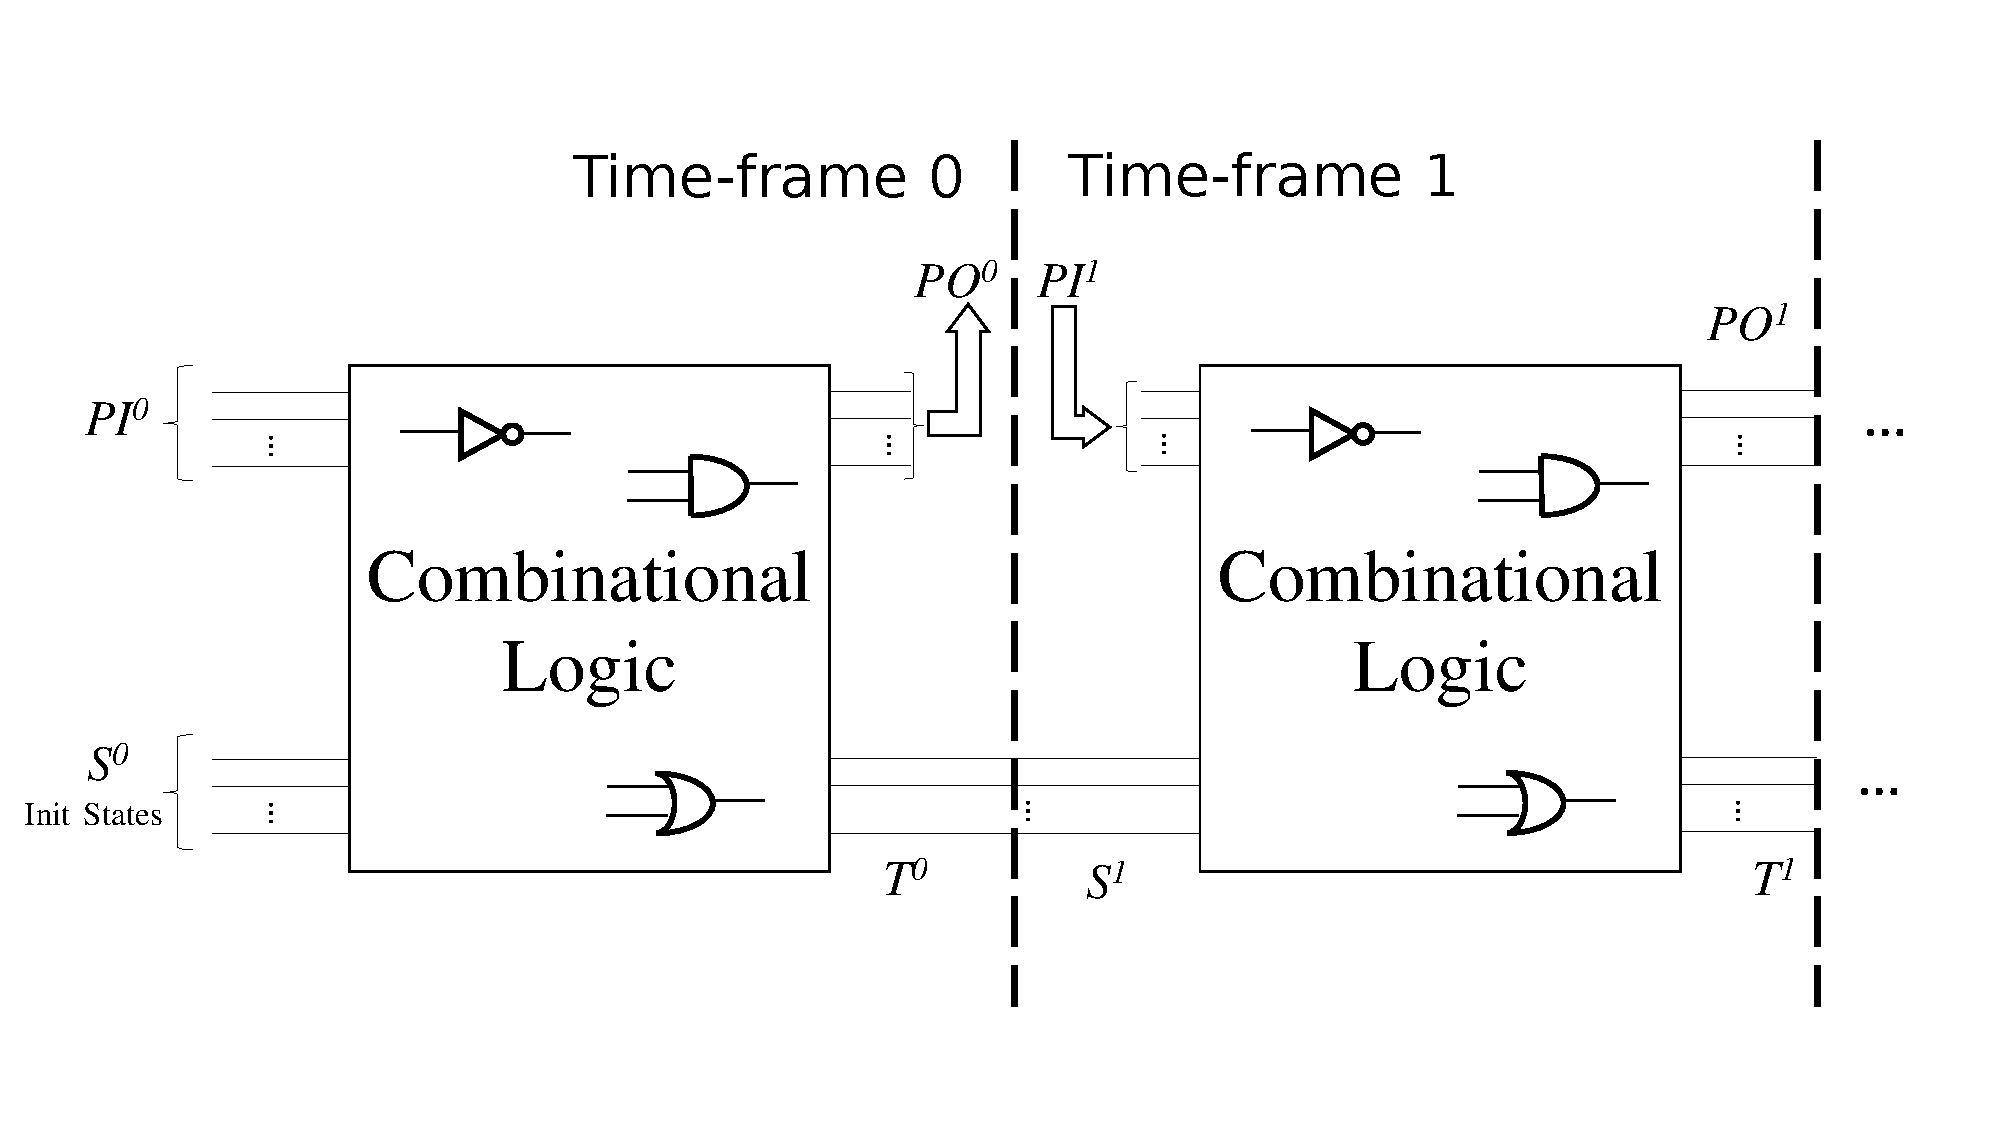
\includegraphics[width=\textwidth]{newfig/unroll.pdf}
}
\caption{The unrolling of a sequential circuit.}
\label{fig:unrolling}
\end{figure}

Unrolling provides a way to transform a sequential circuit into a combinational 
circuit. Therefore,  methods which can be applied to combinational circuit 
verification are also suitable for unrolled sequential circuits. The canonical 
graphical representation of the combinational circuit after unrolling is also 
the canonical representation of the original sequential circuit. For the sequential 
equivalence checking problem, we can also unroll the circuit to be verified and the 
specification to combinational ones, and then perform combinational equivalence checking
techniques \cite{savoj2010combinational}. In the following part we review research and techniques which 
can be applied to unrolled sequential circuits.

\subsection{Canonical Decision Diagrams}
The decision diagrams (DDs) are optimized data structures which can significantly accelerate formal verification.
The most fundamental DD is the Binary DD (BDD), which originates from the 
Shannon's expansion:
\begin{equation}
f(x, y, \dots) = x f_x + x' f_{x'}
\end{equation}
where $f_x = f(x = 1)$ and $f_{x'} = f(x = 0)$ denote the positive and
negative co-factors of $f$ {\it w.r.t.} $x$, respectively.
A BDD is usually represented as a binary tree.
Its ordered and reduced form, the Reduced Ordered Binary Decision Diagram (ROBBD)
\cite{BRYA86}, was the first significant contribution because of its canonicity.  
ROBDDs represent a Boolean function as an
implicit set of points on a canonical directed acyclic graph
(DAG). Manipulation of Boolean functions can then be carried out as
composition operations on their respective DAGs. An example of ROBDD is shown as Figure \ref{fig:BDD}.

Following BDDs,  variants of Shannon's decomposition principle
were explored to develop other functional decision diagrams such as
 FDDs \cite{okfdd}, ADDs \cite{add}, MTBDDs \cite{mtbdd}, and their hybrid 
edge-valued counterparts, HDDs \cite{hdd} and EVBDDs \cite{evbdd}. 
Zero-suppressed BDDs (ZDDs) \cite{minato1993zero,minato1994calculation} use the if-then-else branches
to represent the existence of variables in a cube, and result in lower 
space complexity. They can be used to represent polynomials with integer coefficients.

\begin{figure}[bp]
\centerline{
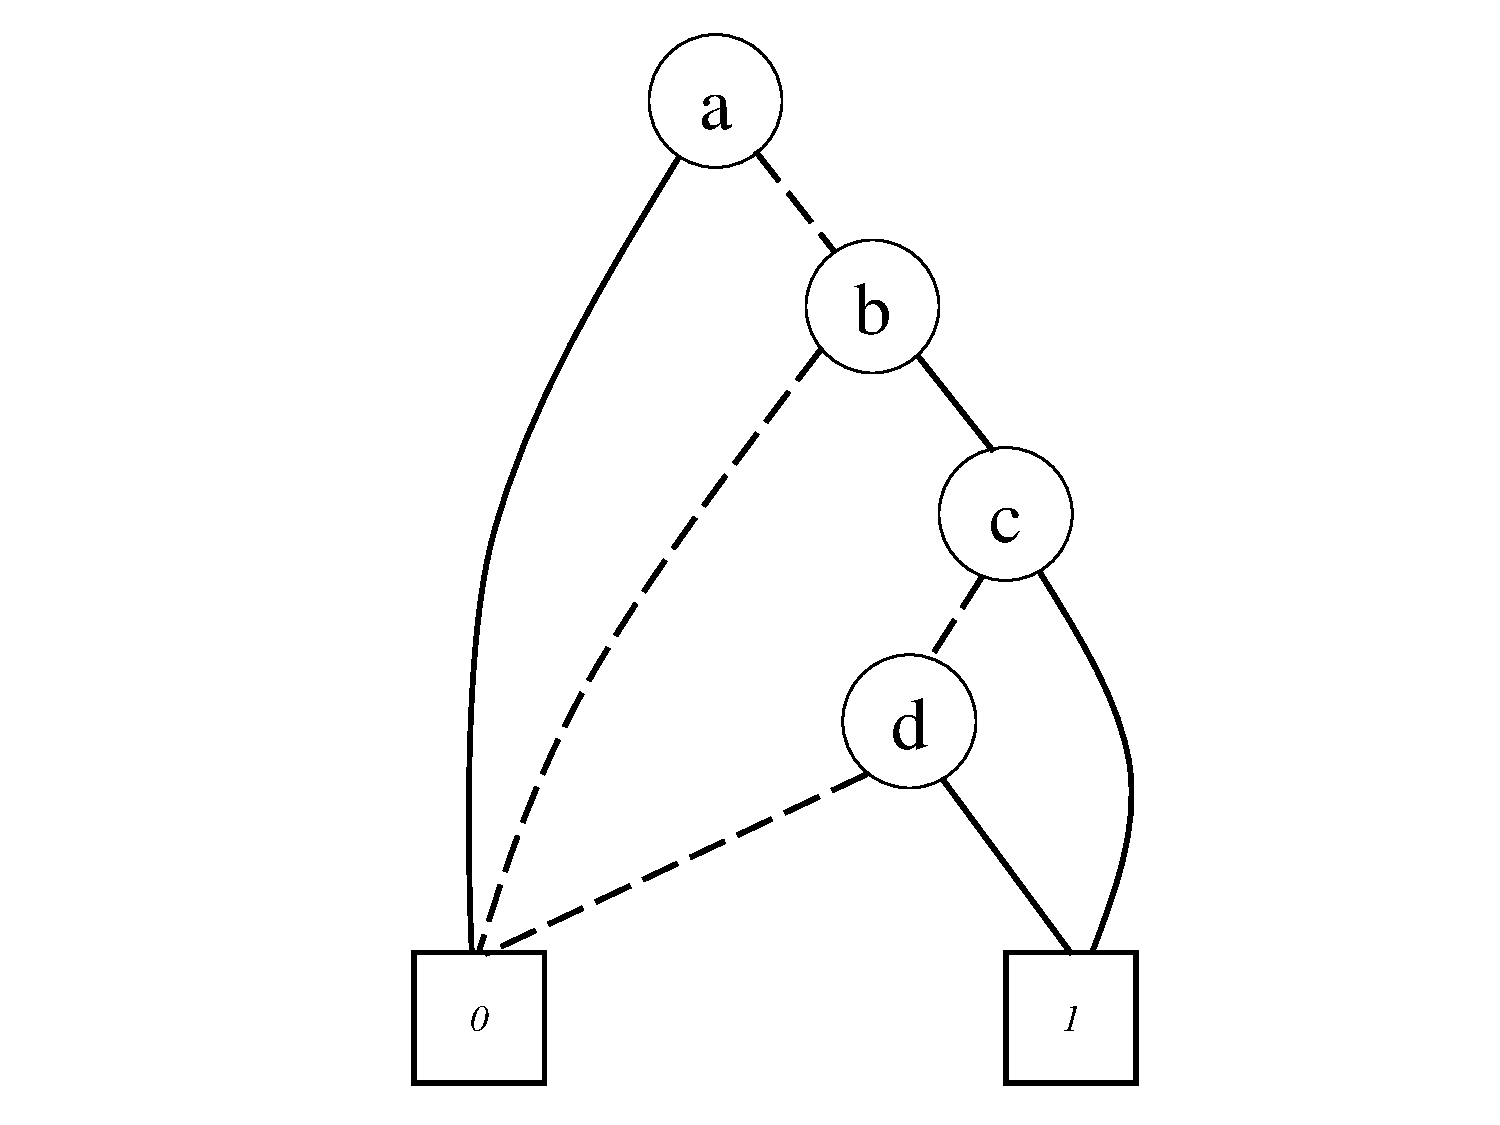
\includegraphics[width=0.45\textwidth]{newfig/BDD.pdf}
}
\caption{ROBDD representing Boolean function $\neg a \land b \land (c\lor d)$ with order $a>b>c>d$.}
\label{fig:BDD}
\end{figure}

The DDs above are all based on bit-level operations. Even in the {\it Word-Level Decision Diagrams}
\cite{WLS}, the decomposition is still point-wise, binary, 
w.r.t. each Boolean variable. These representations do not
serve the purpose of word-level abstraction from bit-level
representations. 

Binary Moment Diagrams (BMDs) \cite{bmd}, and their derivatives K*BMDs
\cite{kbmd} and *PHDDs \cite{phdd}, perform the decomposition of a {\it linear} function
based on its two moments instead of relying on Boolean decomposition. 
MODDs \cite{modd,modd_tcomp} are a DAG representation of the
characteristic function of a circuit over Galois fields $\Fkk$. 
However, MODDs fails to compactly represent large circuits.


Taylor Expansion Diagrams (TEDs) \cite{ted_tcomp} are a
word-level canonical representation of a {\it polynomial expression},
based on the Taylor's series expansion of a polynomial. However, they do
not represent a {\it polynomial function} canonically. 

The use of DDs in traditional formal verification has a lot of advantages. 
For example, DD-based model checking is very efficient as long as the DDs of sequential 
circuit can be setup. The existence of violating states in constructed DDs 
immediately deduces the violation of property. However, when the design gets
larger and larger, the time and space cost of building and storing the diagram 
increases rapidly. In our experiment of verifying a $k$-bit arithmetic circuit 
using ZDDs, when $k$ is larger than 100, the construction of ZDDs occupies 
over $99\%$ runtime of the whole procedure.
\subsection{Combinational Equivalence Checking Techniques}
The CEC problem can be solved using various methods.
Besides using canonical DDs (BDDs
\cite{BRYA86} and their word-level variants \cite{WLS}),
noncanonical representations such as And-Invert-Graph-based (AIG-based) reductions 
\cite{AIG:2002,alanmi:cec:iccad2006} are also very effective. 
Solvers for satisfiability problems (SAT) are good candidates to solve CEC problems,
as long as the miter of two circuits can be described using conjunctive normal form (CNF)
formulas. Applications of SAT on CEC include circuit-SAT solvers \cite{csat}, etc.
If the circuits being compared are structurally highly similar, AIG and circuit-SAT-based
approaches are known to be efficient.
However, when the circuits are functionally equivalent but structurally very dissimilar, none of the 
  contemporary techniques, including quantifier-free bit-vector 
  (QF-BV) theory-based SMT-solvers \cite{Cryptol:fmcad09},
  offer a practical solution.    


Recently integer polynomial based techniques \cite{ciesielski2014function,rolf:date16} have been proposed  to verify the functional 
correctness of integer arithmetic circuits. Their approach formulates the output signature as a polynomial function 
with binary variables and integer coefficients, then rewrites the polynomial by substituting gate output with gate 
inputs. After going through the backward rewriting procedure,  the polynomial
will be composed by only input variables. Then the polynomial is converted to a canonical representation, and compared
with a designated input signature. If they are equivalent, then the arithmetic circuit is successfully verified.
This approach incurs polynomial term explosion during the backward rewriting. The authors proposed a heuristic
to levelize the arithmetic circuit, and substitute several gates' variables at the same time to minimize the risk. However, 
the heuristic proved to be less effective when the inner symmetry of the circuit structure is missing.

% To conclude, automatic formal verification of large {\it
%     custom-designed modulo-arithmetic circuits} largely remains
%   unsolved today.
  
\section{Symbolic Model Checking and Abstraction Refinement}
Model checking is a way to verify certain safety and liveness properties 
in sequential circuits. Symbolic model checking, which avoids using explicit state encoding,
provides more flexibility to reduce the state space and enhance the 
efficiency of model checkers. The implementations of symbolic model checking 
require canonical DDs or SAT solvers \cite{burch1990sequential,burch1991representing,biere1999symbolic}.

Abstraction is a technique to reduce the state space representation by combining states with similar 
characteristics. Sometimes it can effectively lower the number of states that require analysis by orders of magnitude,
without affecting the properties we need to verify. Model checkers then utilize abstracted models 
with interpolation \cite{mcmillan2003interpolation,mcmillan:cav06}.
At first, abstraction was done manually by designers. Clarke {\it et al.} \cite{clarke2000counterexample}
proposed a BDD-based automated abstraction by removing spurious paths from analysis of counterexamples. 
Zhang {\it et al.} \cite{zhang2005design} proposed another abstraction method based on CNF-SAT.
It implemented latch abstraction by removing "irrelevant" latches by analyzing the 
UNSAT core from the $k$-BMC. Jain {\it et al.} \cite{jain2005word} improved the abstraction refinement technique of \cite{clarke2000counterexample},
where they use CNF-SAT to perform the refinement instead of using BDDs. The new approach is applied to verify RTL Verilog
and was known to be successful.

The $k$-BMC with interpolation is a purely incremental model-checking approach, and the interpolation procedure relies
on UNSAT core analysis. To overcome these weaknesses, a hybrid model checker called IC3 is developed 
\cite{bradley2011sat,bradley2011incremental}. IC3 works incrementally to find inductive subclauses
of negations of reached states, meanwhile it is monolithic when computing overapproximations to sets of reachable
states within $1,2,\dots,k$ steps. It is proved to be more efficient than interpolation-based model checking,
although using similar mechanisms.

The above techniques have limitations: they all rely on bit-level information from 
the circuit, which prevents them from being applied to circuits with large datapaths.
Meanwhile, their implementation relies on SAT/BDDs, which is an extension of Boolean 
functions and not compatible with other forms of constraints.

\section{Word-level Techniques Applied to Sequential Circuit Synthesis and Validation}
To better verify word-level designs, word-level verification techniques have been 
explored in recent years. Directly translating bit-vector problems to bit-level 
problems is called {\it bit-blasting}, and usually brings high redundancy and computational complexity in verification.
Attempts to develop pure word-level techniques can be found in
the rich domain of 
theorem proving \cite{arditi:bmd} and bit-vector SMT-solvers
\cite{boolector,cvc3,z3,bitvector98}, automated
decision procedures for Presburger arithmetic \cite{presburger,bultan:mixed_verification}, 
algebraic manipulation techniques 
\cite{devadas:algebraic_manipulation_iccd91}, or the ones based on
term rewriting \cite{AST}, etc.

Polynomial, integer, and other nonlinear representations have also
been researched: Difference Decision Diagrams (DDDs) \cite{ddd-csl99,ddd-mt-98}, interval
diagrams \cite{interval_dd}, interval analysis using polynomials
\cite{polynomial_sanchez99}, {\it etc.} Most of these have found 
application in constraint satisfaction for simulation-based
validation:  \cite{Ritter99,hsat,lpsat,brinkmann:asp-dac,Huang:tcad01,bitvector98}. Among
these, \cite{brinkmann:asp-dac,Huang:tcad01,bitvector98}
have been used to {\it solve} integer modular arithmetic on linear
expressions -- a different application from {\it representing}
finite field modulo-arithmetic on polynomials in a canonical form.   

Uninterpreted function abstraction is also an important category of 
word-level techniques which facilitates word-level model checking.
Usually uninterpreted symbols have no notion of bit-vector-precision. However, these techniques
constrain them 
using functional consistency among the evaluations of word variables
\cite{UF1,UF2,UF3}.


\section{Verification Using Algebraic Geometry}

Symbolic computer algebra techniques have been employed for formal
verification of circuits over $\Z_{2^k}$ and also over
Galois fields $\Fkk$. 
Verification techniques using Gr\"obner bases
\cite{Avrunin:CAV,gbverify:2007,manna:program} are proposed,
but they do not address the problem of high computational complexity to
compute Gr\"obner bases.

Verification of a combinational Galois field arithmetic circuit $C$ against a
polynomial specification $\Func$ has been previously addressed 
\cite{ibm:blueveri,lv:tcad2013,pruss:dac14}. Verification problems in
\cite{ibm:blueveri,lv:tcad2013} are formulated using
Nullstellensatz and decided using the \Grobner basis algorithm.

The paper 
\cite{pruss:dac14} performs verification by deriving a canonical
word-level polynomial representation $\Func$ from the circuit $C$. Their
approach views any arbitrary Boolean function (circuit) $f: \B^k
\rightarrow \B^k$ as a polynomial function $f: \Fkk \rightarrow \Fkk$,
and derives a canonical polynomial representation $\Func$ over
$\Fkk$. They show that this can be achieved by computing a reduced 
\Grobner basis {\it w.r.t.} an {\it abstraction term order} derived from the
circuit. Subsequently, they propose a \underline{r}efinement of this
\underline{a}bstraction \underline{t}erm \underline{o}rder (called
RATO) that enables them to compute the \Grobner basis of a smaller subset
of polynomials. The authors show that their approach can prove the
correctness of up to 571-bit combinational GF multipliers. 

IBM proposed a method to apply algebraic geometry techniques 
to verifying error coding circuits \cite{BLUEVERI}.
Recent papers \cite{rolf:date16,rolf:FMCAD16} provide a way to utilize 
algebraic geometry and GB-based symbolic computing and perform 
equivalence checking on integer arithmetic circuits and floating-point 
arithmetic circuits, respectively.

The use of algebraic geometry
for sequential circuit verification and symbolic model checking has
been presented before. Avrunin presented the
concept of symbolic MC using algebraic geometry in
\cite{Avrunin:CAV}. Later, in \cite{vardi-iasted07}, Vardi presented
GB-algorithms for CTL, LTL, and 
bounded MC over Boolean rings. However, these approaches are a
straightforward transformation of the problem to {\it bit-level}
Boolean GB engines which are used in lieu of BDDs or SAT solvers. All
the concepts of word-level reachability, abstraction-refinement using
interpolation or UNSAT cores, etc., that we desire were not the focus of
\cite{Avrunin:CAV,vardi-iasted07}. 

\section{Concluding Remarks}
From the investigation of previous work, techniques are to be researched that 
can perform the FSM traversal at word level to verify a property excluding spurious 
faults. Meanwhile, many abstraction refinement techniques utilize information from UNSAT cores.
We propose to solve these problems in the context of word-level verification,
with data representation, abstraction, and algorithm execution all carried out 
at word level.

In this dissertation, we propose a purely word-level reachability analysis approach, which has never been done before.
We achieve this by modeling the transition relations, states and the traversal algorithm at word level.
We borrow inspirations from \cite{tim:phd,gao:qe-gf-gb} to perform state space abstraction.
Moreover, we demonstrate applications of our proposed approach to sequential arithmetic verification, which has 
not been done before, either.
Finally, we show algebraic geometry analogs of UNSAT cores of polynomial ideals, and describe algorithms
to extract and refine these cores.

\section{Sequential GF Multiplier Design}
\label{sec:design}

Let us briefly describe the fundamentals behind the design of normal
basis sequential GF multipliers, so as to put in perspective the type
of designs that have been verified in this paper. Let $R =
\sum_{i=0}^{k-1} r_i \beta^{2^{i}}, ~A = \sum_{i=0}^{k-1} a_i
\beta^{2^{i}}, ~B = \sum_{i=0}^{k-1} b_i \beta^{2^{i}}$, then 
\[
R = A\cdot B = (\sum_{i=0}^{k-1} a_i \beta^{2^{i}}) (\sum_{j=0}^{k-1}
b_j \beta^{2^{j}})  =
\sum_{i=0}^{k-1}\sum_{j=0}^{k-1}a_ib_j\beta^{2^i}\beta^{2^j}\nonumber 
\]

The expressions $\beta^{2^i}\beta^{2^j}$ are called cross-product
terms and they can also be represented in normal basis: 
\begin{displaymath}
\beta^{2^i}\beta^{2^j} =
\sum_{n=0}^{k-1}\lambda_{ij}^{(n)}\beta^{2^n}, \ \ \lambda_{ij}^{(n)}
\in \Ftwo. 
\end{displaymath}

From the above two equations, one can see that the expression for the
$n^{th}$ digit of product $R = (r_0, \dots, r_n, \dots r_{k-1})$ is:
\[
r_n = \sum_{i=0}^{k-1}\sum_{j=0}^{k-1}\lambda_{ij}^{(n)}a_ib_j = A
\cdot M_n \cdot B^T, ~~0 \leq n \leq k-1
\]

where $M_n = (\lambda_{ij}^{(n)})$ is a binary $k \times k$ matrix over
$\Ftwo$, and it is called the $\lambda$-matrix. 
%The collection of all
%$\{M_n\}$  $\lambda$-matrices is called the multiplication
%table. 
Moreover, let $r_n = A \cdot M^{(n)} \cdot B^T$.
Then $r_{n-1} = A \cdot M^{(n-1)} \cdot B^T = rotate(A) \cdot M^{(n)}
\cdot rotate(B)^T$. This implies that $M^{(n)}$ is generated by right
and down cyclic shifting $M^{(n-1)}$. Therefore, the hardware design
of sequential GF multipliers is based on mappings of $A\cdot M_n
\cdot B^T$ into AND-XOR gates and cyclic shift operations. 

This paper verifies the implementation of two distinct 
architectures of {\it sequential multipliers with parallel output
  (SMPO)}, namely: i) the Agnew-SMPO  \cite{agnew1991implementation}
by G. B. Agnew, which is a straight-forward implementation of the
$\lambda$-matrix; and ii) the more recent, more complicated, yet very
efficient RH-SMPO \cite{RHmulti}, by Reyhani-Masoleh and Hasan,
depicted in Fig. \ref{fig:RHmulti}.  

\begin{figure}[hbt]
\centering{
%\begin{minipage}{12cm}
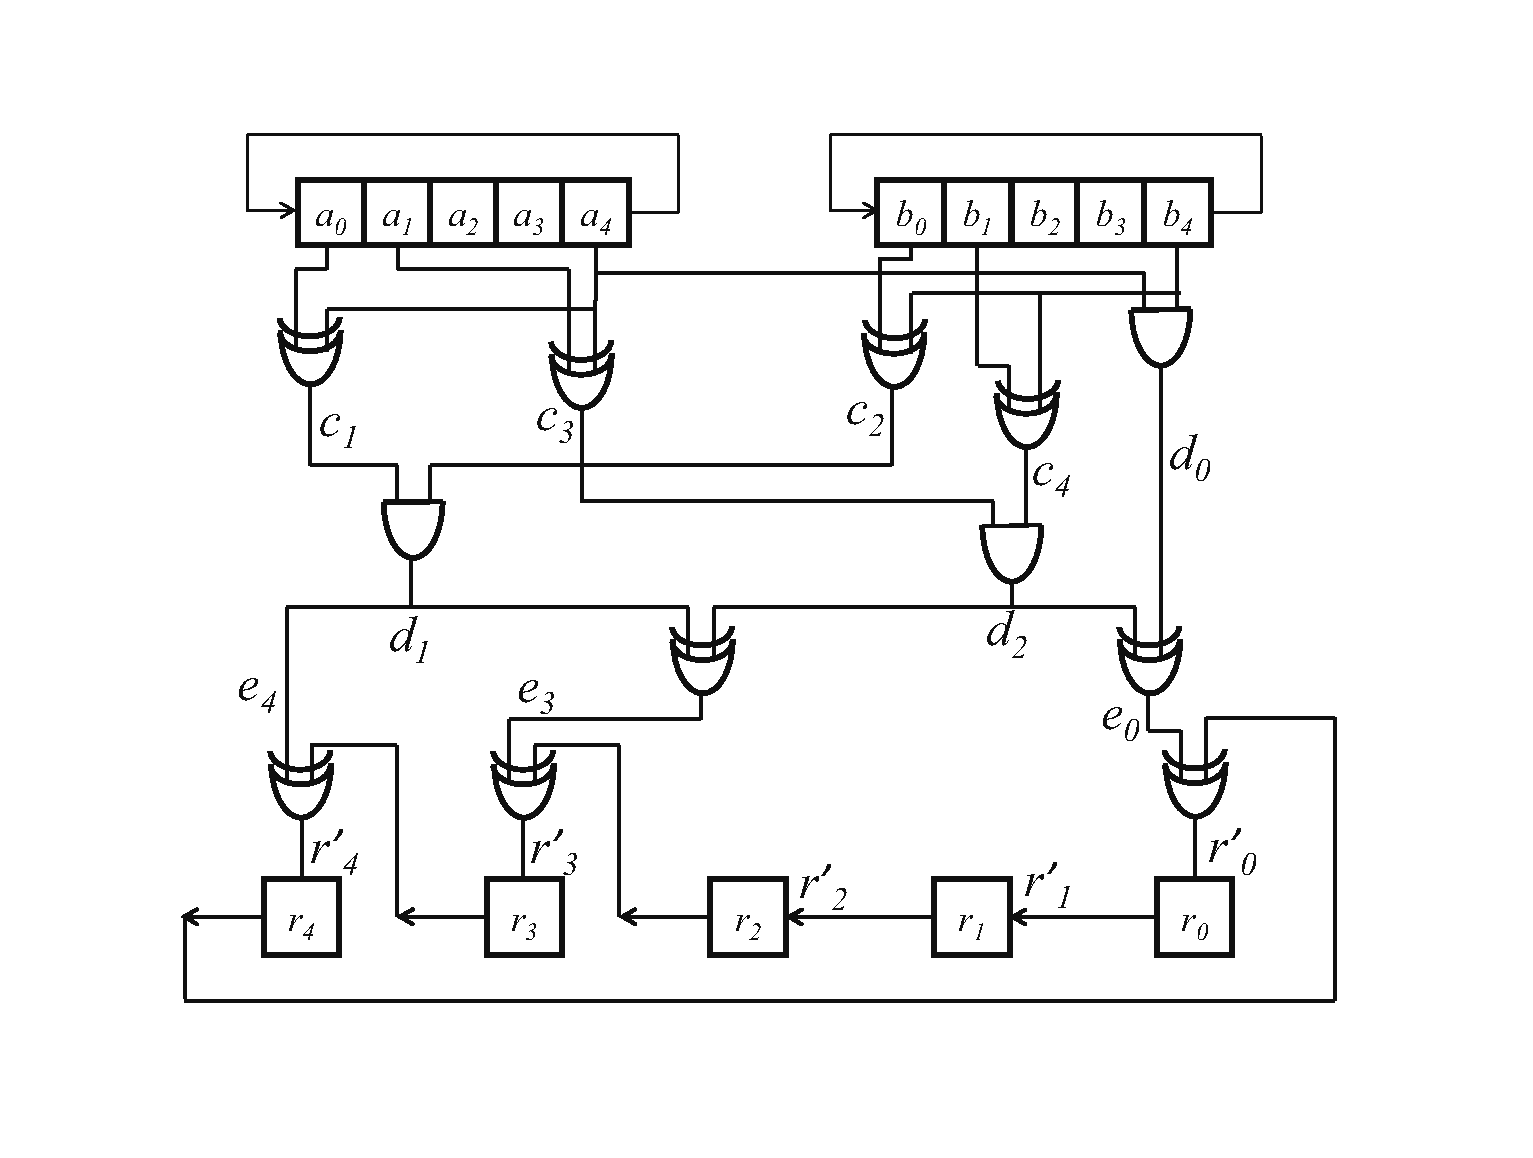
\includegraphics[width=4in]{./RH.eps}
\vspace{-0.2in}
\caption{A 5-bit Reyhani-Hasan Sequential Multiplier with Parallel Outputs (RH SMPO)}
%\end{minipage}
\label{fig:RHmulti}}
\end{figure}

%\input{myformulae.tex}


\section{Preliminaries}

\subsection{FSM model for sequential circuits}
A finite state machine (FSM) is a mathematical model of computation for designing and analyzing sequential logic 
circuits. If a FSM's primary outputs depend on primary inputs and present state inputs, it is named as a \textit{Mealy machine};
the formal definition is as follows:
\begin{Definition}
A Mealy machine is an $n$-tuple $\mathcal M = (\Sigma,O,S,S^0,\Delta,\Lambda)$ where
\begin{itemize}
\item $\Sigma$ is the input label, $O$ is the output label;
\item $S$ is the set of states, $S^0\subseteq S$ is the set of initial states;
\item $\Delta:\ S\times\Sigma\to S$ is the next state transition function;
\item $\Lambda:\ S\times\Sigma\to O$ is the output function.
\end{itemize}
\end{Definition}
The other kind of FSM is \textit{Moore machine}, its difference from Mealy machine is that
its primary outputs only depend on the present states, i.e. the output function is defined as
$$\Lambda:\ S \to O$$
Typical sequential circuits can be depicted as Fig.\ref{fig:seqmodel}(a). Primary inputs
$x_1,\dots,x_m \in \Sigma$, and primary outputs $z_1,\dots,z_n\in O$. Signals $s_1,\dots,s_k$ 
are present state (PS) variables, $t_1,\dots,t_k$ are next state (NS) variables.
We can define 2 $k$-bit words denoting the PS/NS variables as there are $k$ flip-flops
in the datapath: $S = (s_1,\dots,s_k), ~T=(t_1,\dots,t_k)$. Transition function
at bit level are defined as $\Delta_i: t_i = \Delta_i(s_1,\dots,s_k,x_1,\dots,x_m)$.
\begin{figure}[hbt]
\centering{
%\begin{minipage}{12cm}
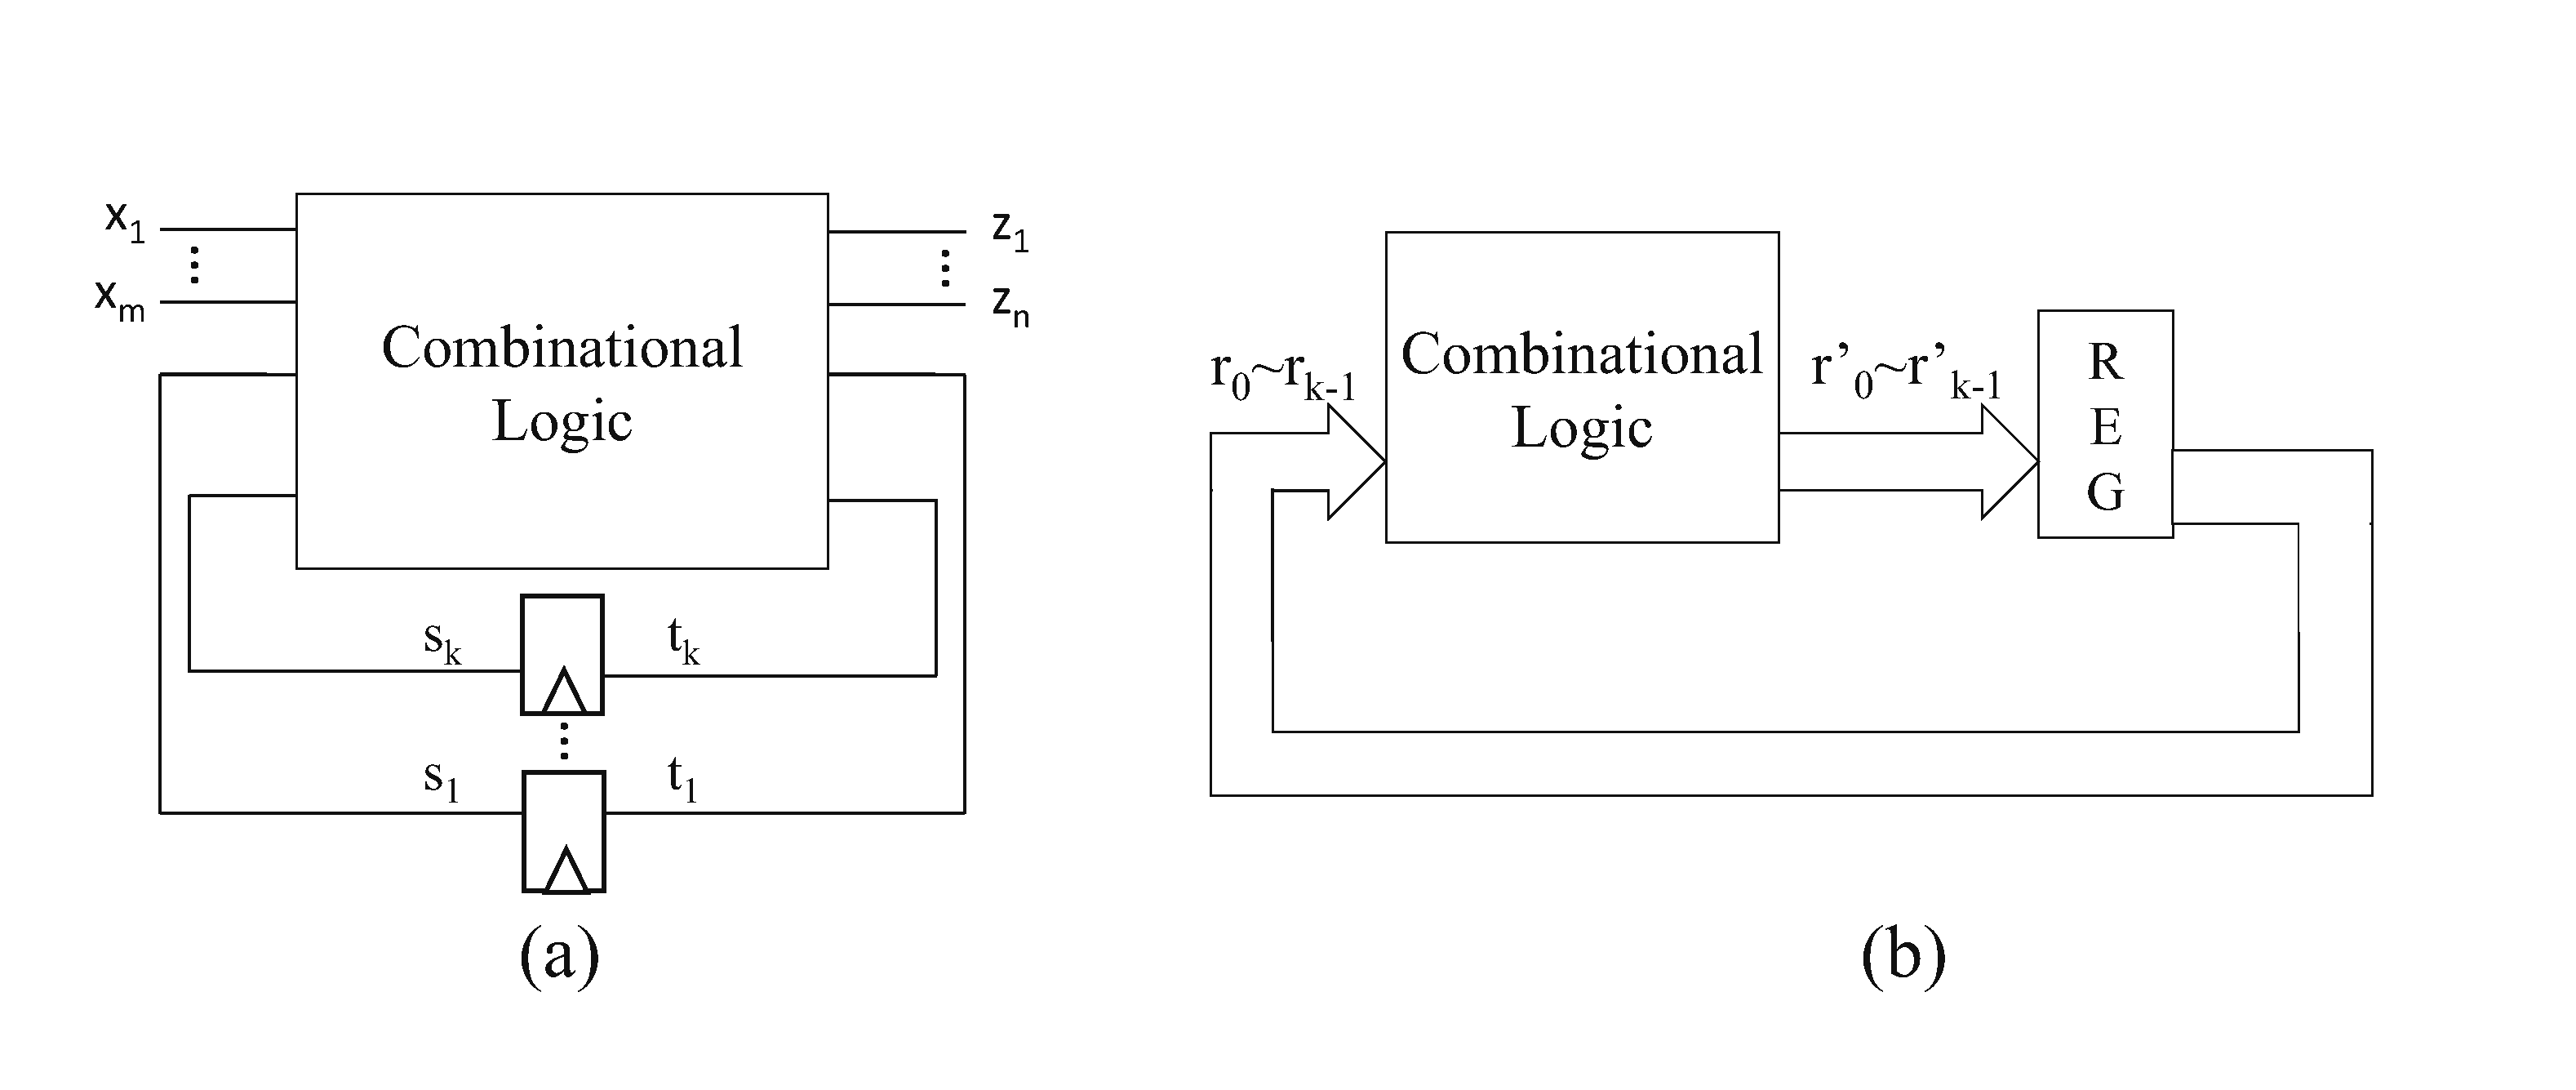
\includegraphics[width=3.5in]{./seqmodel.eps}
% \vspace{-0.2in}
\caption{FSM models of sequential circuits}
%\end{minipage}
\label{fig:seqmodel}}
\end{figure}
In some cases, arithmetic computations are implemented as Moore machines where input operands
are loaded into register files $R$ and the FSM is executed for $k$ clock cycles.
We can simplify them to the model in Fig.\ref{fig:seqmodel}(b).

\subsection{Commutative algebra and algebraic geometry preliminaries}
A {\bf field} $\mathbb{F}$ is a set of elements, including 0 and 1 (unity),
allowing for associative and commutative addition and multiplication;
and every non-zero element has a multiplicative inverse.  A {\bf
  finite field} or {\bf Galois filed} is a field with a finite number
($q$) of elements, and is denoted by $\Fq$, where $q=p^k$ is a power of
a prime integer $p$. In our work, $q = 2^k$ for
a given $k$, where $k$ represents the datapath (bit-vector)
word-lengths, or the number of memory elements (state registers) in
finite state machines. 

Let the field $\mathbb{F}_2 = \{0, 1\} ~(\equiv \B)$, and let
$\mathbb{F}_2[X]$ denote the set (ring) of all univariate polynomials
in variable $X$ with coefficients from $\mathbb{F}_2$. Then, the
Galois field $\Fkk$ is constructed as $\Fkk = \mathbb{F}_2[X] \pmod{
  P(X)}$, where $P(X)$ is an irreducible polynomial over
$\mathbb{F}_2$. Let $\alpha$ be a root of the irreducible polynomial
$P(X)$, i.e. $P(\alpha) = 0$. Any element $A \in \Fkk$ can be
represented as $A = \sum_{i=0}^{k-1} a_i \alpha^i$, where $a_i \in
\mathbb{F}_2$. The field $\Fkk$ is therefore, a $k$-dimensional {\it
  extension} of the base field $\mathbb{F}_2$: so,  $\mathbf{\Fkk \supset
\mathbb{F}_2}$. Consequently, all operations of addition and
multiplication in $\Fkk$ are performed modulo the irreducible
polynomial $P(\alpha)$ and coefficients are reduced modulo 2.  

Boolean variables in field $\mathbb B$ can be easily mapped to
elements in $\mathbb F_2$. Since $\mathbb F_2 \subset \Fkk$, these 
%Namely $k$-bit Boolean bit-vector defined
%over Boolean ring $\mathbb B^k$ can also be mapped uniquely  to $\Fkk
%= \mathbb F_2[x_1,\dots,x_k]$. 
Boolean operators are interpreted as functions over $\Fkk$ (where $+$
and $\cdot$ are addition and multiplication performed modulo 2): 
\begin{align*}
&a\land b \to a\cdot b\\
&a\oplus b \to a+b\\
&\neg a \to 1+a\\
&a \bar{\oplus} b \to 1+a+b\\
&a \lor b \to a+b+a\cdot b
\end{align*}

Using these mappings we can write Boolean functions in form of
polynomials over $\mathbb F_2\subset \Fkk$. 
These concepts provide a mechanism to represent and
manipulate both bit-level ($\mathbb{F}_2$) and $k$-bit word-level
constraints {\bf in one unified mathematical domain $\Fkk$ --- a
  concept we   exploit for abstraction. }
  Consider Ex.\ref{ex:motiv},
polynomials for transition functions (bit-level outputs) $f_1,f_2$
are over $\mathbb F_2$, i.e. $f_1,f_2\subseteq \mathbb F_2 \subset \Fkk$,
and polynomials containing word-level variables $f_3,f_4,f_5 \subseteq \Fkk$.
All polynomials belong to unified domain $f_1,f_2,\dots,f_5 \subseteq \Fkk$.

It is well-known that every Boolean mapping between $k$ dimensional
Boolean spaces $f: \B^k \rightarrow \B^k$ can be construed as a
function over Galois fields $f: \Fkk \rightarrow \Fkk$. Moreover,
every function $f: \Fkk \rightarrow \Fkk$ is a polynomial function: 
i.e. $f$ can be represented by way of a unique, minimal, canonical
polynomial $\F(X)$, and the work of \cite{timDAC} shows how to
efficiently derive such polynomial representations from circuits ---
another concept that makes our approach feasible. 


We represent Boolean circuits by way of polynomials over
$\Fkk$. If we take indeterminates $x_1,x_2,\dots,x_n$, an arbitrary
combination of their finite product  
$x_1^{d_1}\cdot x_2^{d_2}\cdots x_n^{d_n}, d_i\geq 0$ 
is a {\bf monomial}. A {\bf polynomial} $f = c_1 X_1 + c_2 X_2 + \dots
+ c_t X_t$ is a finite sum of terms, where $c_1, \dots, c_t$ are
coefficients and $X_1, \dots, X_t$ are monomials. The set of {\it all}
such polynomials with coefficients from $\Fkk$ forms a {\bf
  multivariate polynomial ring} denoted $\Fkk[x_1,\dots,x_n]$. 
A monomial ordering $X_1 > X_2 \dots > X_t$ is imposed on the
polynomials to process them systematically. Then, $LT(f) = c_1 X_1,
LM(f) = X_1$ denote the leading term and the leading monomial of $f$,
respectively. 


Multivariate polynomial division will play a key role in our
algorithmic techniques. Division is implemented as {\it cancellation
  of terms.} Given polynomials $f, g$, if $cX$ is a term in
$f$ that is divisible by $LT(g)$, then $f \xrightarrow{g} r$ denotes a
one-step reduction (division) of $f$ by $g$, resulting in remainder $r
= f - {{cX} \over {LT(g)}} \cdot g$. This has the effect of cancelling
the term $cX$ from $f$. 
\begin{Example}
\label{ex:multidiv}
If $f = e + cd$ and $g = c + ab$,
then the term $cd$ in $f$ can be canceled by $LT(g) = c$: $r = f - {cd
  \over c} g = e + abd$. 
\end{Example}
  Similarly, $f$ reduces to $r$ modulo the set
of polynomials $F = \{f_1, \dots, f_s\}$, denoted $f \stackrel{F}
{\textstyle   \longrightarrow}_+ r$, such that no term in $r$ is
divisible (cancellable) by the $LT(f_i)$ of any polynomial in $ f_i
\in F$.    


In verification, we have to analyze the {\it solutions to a
set of polynomials.} The set of all solutions to a system of
polynomial equations $f_1 = \dots = f_s = 0$ is defined as the affine variety:
\begin{Definition}
Given a set of polynomials $f_1,\dots,f_s$ over ring $\mathbb F_q[x_1,\dots,x_n]$, their 
{\bf affine variety} 
$$V(f_1,\dots,f_s) = \{(a_1,\dots,a_n)\in  (\mathbb F_q)^n |
f_1(a_1,\dots,a_n) = \cdots = f_s(a_1,\dots,a_n) = 0\}$$ 
\end{Definition}

Generally we can find many sets of polynomials with the same variety, which are linear combinations
of given set of polynomials. This set is defined as follows:
\begin{Definition}
{\bf Ideal of Polynomials:} Let $f_1,f_2,\dots,f_s\in \mathbb F[x_1,\dots,x_n]$.
Define an ideal
$$J = \langle f_1,f_2,\dots,f_s\rangle = \{f_1\cdot h_1 + f_2\cdot h_2 +\cdots + f_s\cdot h_s : h_1,\dots,h_s\in \mathbb F[x_1,\dots,x_n]\}$$
We call $J = \langle f_1,f_2,\dots,f_s\rangle$ an ideal generated by $f_1,\dots,f_s$ and these polynomials 
the {\bf generators} of ideal $J$.
\end{Definition}
% On the other hand, if given another polynomial $f$, we need to judge whether it belongs to $J$.
A practical problem is: given an ideal $J = \langle f_1,f_2,\dots,f_s\rangle$ and a polynomial $f$,
we need to check if the variety of $J$ can make the evaluation of $f$ equal to 0, i.e. $f$ vanishes on $V(J)$.
This problem is usually described as ideal membership checking problem.
\begin{Definition}
{\bf Ideal membership:} Let $f_1,f_2,\dots,f_s\in \mathbb F[x_1,\dots,x_n]$, and $J = \langle f_1,f_2,\dots,f_s\rangle$
be an ideal over ring $\mathbb F[x_1,\dots,x_n]$. If 
$$f = f_1h_1 + f_2h_2 + \cdots + f_sh_s$$
then $f\in J$.
\end{Definition}

An ideal may have many generating sets. For example, we may have different set of polynomial generators denoting
the same ideal, where they have the same variety: $\langle f_1,\dots,f_s\rangle = \langle h_1,\dots,h_r\rangle
= \langle g_1,\dots,g_t\rangle$ such that $V(f_1,\dots,f_s) = V(h_1,\dots,h_r) = V(g_1,\dots,g_t)$.
Therefore a canonical representation of an ideal is needed, which leads to the concept of Gr\"obner bases.

\begin{Definition}
The set $G = \{g_1, \dots,
g_t\}$ is called a \textbf{\Grobner basis} of $J$ if and only if the
leading term of all polynomials in $J$ is divisible be the leading
term of some polynomial $g_i$ in $G$: i.e. $\forall f \in J, \exists
g_i \in G \ s.t. \ LT(g_i) ~|~ LT(f)$. 
\end{Definition}
% The famous Buchberger's
% algorithm, given in textbook \cite{ideals:book}, is used to compute a
% \Grobner basis (GB). Operating on  input $F = \{f_1, \dots, f_s\}$,
% and subject to the imposed term order $>$, it derives $G = GB(J) = \{
% g_1, \dots, g_t \}$. Buchberger's algorithm repeatedly computes
% $S$-polynomials. For pairs $(f_i, f_j) \in F$, $Spoly(f_i, f_j) =
% \frac{L}{lt(f_i)}\cdot f_i - \frac{L}{lt(f_j)}\cdot f_j$, where $L =
% LCM(LM(f_i), LM(f_j))$. Reducing $Spoly(f_i, f_j) \xrightarrow{F}_+ r$
% cancels the leading terms of $f_i, f_j$ and gives a polynomial $r$
% with a new leading term. This remainder $r$ is added to the current
% basis and $Spoly(f_i, f_j)$ computations are repeated for all pairs of
% polynomials until all $S$-polynomials reduce to 0.  

An advantage of representing an ideal with GB is that it can serve as a decision procedure for ideal membership
test when dividing a polynomial $f$ by a GB, i.e.
$$G = GB(J) \Longleftrightarrow \forall f\in J, f\xrightarrow{g_1,g_2,\dots,g_t}_{+} 0$$
Gr\"obner basis can be reduced by eliminating redundant elements. \textbf{A reduced GB is a canonical representation of 
the ideal under a given monomial ordering}. Given an ideal $J = \langle f_1,\dots,f_s\rangle, ~G = 
\{g_1,\dots,g_t\}$ is the GB of $J$, it can be computed by Buchberger's algorithm (refer to textbook \cite{ideal:book}).

Another advantage of using GB representation is that GB computation can work as a {\it quantification procedure}.
In the following part we will introduce the concept of \textit{vanishing polynomials}, \textit{elimination ideal}, etc.
as the bases of this theory.

{\it Fermat's little theorem over $\Fq$:} For any $ \alpha \in \mathbb
F_{q}, \alpha^q = \alpha$. Therefore, the polynomial $x^q - x$
vanishes ($=0$) over $\Fq$, and is called a vanishing polynomial. We
denote by $J_0 = \langle x_1^q - x_1, \dots, x_d^q - x_d \rangle$ the
ideal of all vanishing polynomials in $\Fq[x_1, \dots, x_d]$. When $q
= 2^k, x^q - x = x^q + x$ as $-1 = +1$ over $\Fkk$.

Gr\"obner bases can be used to {\it eliminate} (i.e. quantify) variables from an
ideal. Given ideal $J = \langle f_1,\dots,f_s\rangle \subset \mathbb
F_{q}[x_1,\dots,x_d]$, the $l^{th}$ elimination ideal $J_l$ is the
ideal of $\Fq[x_{l+1}, \dots, x_d]$ defined by $J_l = J \cap
\Fq[x_{l+1}, \dots, x_d]$. Variable elimination can be achieved 
by computing a Gr\"obner basis of $J$ w.r.t. elimination orders: 
\begin{Theorem}
\label{thm:elim}
(Elimination theorem\cite{ideals:book}) Let $J\subset \mathbb
  F_{2^k}[x_1,\dots,x_d]$ be an ideal and let $G$ be a Gr\"obner basis
  of $J$ with respect to a lexicographic (LEX) ordering where
  $x_1>x_2>\cdots>x_d$. Then for every $0\leq l\leq d$, the set $G_l =
  G\cap\mathbb F_{2^k}[x_{l+1},\dots,x_d]$ is a Gr\"obner basis of
  the $l$-th elimination ideal $J_l$.
\end{Theorem}
We describe an application of elimination ideals using following example borrowed from \cite{ideals:book}:
\begin{Example}
Consider polynomials $f_1: x^2-y-z-1;\ f_2:x-y^2-z-1;\ f_3:x-y-z^2-1$ and ideal $J = \langle f_1,f_2,f_3\rangle
\subset \mathbb C[x,y,z]$. Gr\"obner basis $G = GB(J)$ w.r.t. LEX term order equals to 
$g_1:x-y-z^2-1;\ g_2:y^2-y-z^2-z;\ g_3: 2yz^2-z^4-z^2;\ g_4:z^6-4z^4-4z^3-z^2$. From observation,
we find that the polynomial $g_4$ only contains variable $z$ ($x,y$ eliminated), and polynomials $g_2,g_3,g_4$ only contain variables
$y,z$ ($x$ eliminated). According to theorem \ref{thm:elim}, $G_1 = G\cap\mathbb C[y,z] = \{g_2,g_3,g_4\}$
is the Gr\"obner basis of the $1^{st}$ elimination ideal of $J$ and $G_2 = G\cap\mathbb C[z] = \{g_4\}$ is the 
$2^{nd}$ elimination ideal of $J$, respectively.
\end{Example}

\subsection{Application of elimination theorem on circuit verification}
\label{sec:elim}
Assume that we are given a circuit (combinational component) with input $A = (a_0,\dots,a_{k-1})$ and output 
$R = (r_0,\dots,r_{k-1})$ (both can be represented
by word level variables in $\Fkk$). We can describe this circuit with an elimination ideal $J+J_0$, where
$J$ is the ideal generated by the polynomials corresponding to circuit gates and $J_0$ is the ideal of vanishing polynomials.
The authors of \cite{timDAC} showed that for any combinational
logic block, a canonical word-level polynomial representation can be
derived through \Grobner bases computed with elimination orders:
\begin{Lemma}
(From \cite{timDAC}) Given a combinational circuit $C$ with $k$-bit
  input $A = (a_0, \dots, a_{k-1})$ and $k$-bit output $R = (r_0, \dots,
  r_{k-1})$. Denote by $x_1, \dots, x_d$ all the bit-level
  variables of   $C$. Let $J = \langle f_1, \dots, f_s \rangle \subset
  \Fkk[x_1, \dots, x_d, R, A]$ denote all the polynomials corresponding to the
  logic gates of the circuit. Let $J_0 = \langle x_1^2 - x_1, \dots,
  x_d^2 - x_d, R^q - R, A^q - A \rangle$ be the vanishing ideal, so
  that $J + J_0 = \langle f_1, \dots, f_s, ~~ x_1^2 - x_1, \dots,
  x_d^2 - x_d, R^q - R, A^q - A \rangle$. Compute \Grobner basis $G =
  GB(J + J_0)$ w.r.t. lex term order with $x_1 > x_2 > \dots > x_d > R
  > A$. Then $G_d = G \cap \Fkk[R, A]$ eliminates the internal
  variables $x_1, \dots, x_d$ of the circuit. $G_d$ also contains the
  word-level polynomial $R = \F(A)$ which canonically represents the
  function of the circuit with only word level variables $R$ and $A$.
\end{Lemma}
This lemma shows an application of GB computations over an elimination ideal.
Since it abstracts the function of a combinational circuit, we call the term order
$primary~inputs~and~intermediate~variables~>~word~level~output~>~word~level~inputs$
as \textit{abstraction term order} (ATO).
If we further eliminate word-level input, the result will be a polynomial containing only 
the word-level output variable. In a sequential circuit
such as Ex.\ref{ex:motiv}, the output of combinational logic serves as the next state variable. Polynomial $g_T$ in
the example is the desired projection; i.e. using GB computation on elimination ideal and eliminating to NS
variables provides us the canonical representation of reachable states in next time frame.



% Machine traversal is key for many verification techniques, e.g. to check
% the equivalence of 2 FSMs, we can observe whether the output responses are the same at
% every step of traversal. An explicit traversal is usually infeasible, here we use 
% implicit state enumeration (BFS traversal) based on Boolean formulas to implement a machine traversal.
% The algorithm is as follows:
% \begin{algorithm}[hbt]
% \SetAlgoNoLine
%  \KwIn{Transition functions $\Delta$, initial state $S^0$}
% 
%   $from^0 = reached = S^0$\;
%   \Repeat{$new^i == 0$}
%   {
%   	$i \gets i + 1$\;
% 	$to^i \gets$Img$(\Delta, from^{i-1})$\;
% 	$new^i \gets to^i \cap \overline{reached}$\;
%   	$reached \gets reached \cup new^i$\;
% 	$from^i \gets new^i$\;
%   }
% \Return{$reached$}
% \caption {Breadth-first Traversal Algorithm for Reachability Analysis of FSMs}\label{alg:BFS}
% \end{algorithm}
% The main computation in this algorithm is the \textit{image function}. Img$(\Delta,from^{i-1})$
% denotes the forward image of the set $from^{i-1}$ under the transition function $\Delta$.
% Let  $\Delta_i$ denote the transition relation 
% for $i^{th}$ bit of output $T$ (denoted by $t_i$), and it is described by a Boolean function. We can obtain the transition relation 
% for bit-vector $T$: $Tran(s_0,s_1,x,t_0,t_1) = \bigwedge_{i=1}^{2}(t_i\ \bar{\oplus}\ \Delta_i)$. Assume present states
% are represent by Boolean formulas $PS(s_0,s_1)$, then the image function is written as
% $\text{Img}(Tran,\ PS) = \exists_{s_0,s_1}\exists_{x}[Tran(s_0,s_1,x,t_0,t_1)\land PS(s_0,s_1)]$, where
% $\exists_x f$ denotes the existential quantification of $f$ w.r.t. $x$.
% \begin{Example}
% We use implicit state enumeration based on Boolean formulas to traverse FSM in Fig.\ref{fig:fsm}.
% Initial state $\{00\}$ can be represented by Boolean formula $C(s) = \overline{s_0}\cdot \overline{s_1}$.
% Transition function for $NS$ variables are 
% $$t_0\overline{\oplus}\Delta_0 = t_0\overline{\oplus}(\overline{x}\overline{s_0}\overline{s_1}+s_0s_1)$$
% $$t_1\overline{\oplus}\Delta_1 = t_1\overline{\oplus}(x\overline{s_0}+s_0\overline{s_1})$$
% \end{Example}
\section{Verification of Sequential GF Circuits}
\label{sec:theory}

We follow  the sequential GF circuit model of
Fig. \ref{fig:sequential}, with word-level variables $A, B, R$
denoting {\it present states (PS)} and $A', B', R'$ denoting {\it next
  states (NS)} of the machine; where $A = \sum_{i=0}^{k-1} a_i \beta^{2^i}$
for the PS variables and $A' = \sum_{i=0}^{k-1} a_i'
\beta^{2^i}$ for NS variables, and so on. The normal element $\beta$ is
given. Variables $R (R')$ correspond to those that 
store the result, and $A, B (A', B')$ store input operands. {\it E.g.,}
for a GF multiplier, $A_{init}, B_{init}$ (and $R_{init} =
0$) are the initial values (operands) loaded into the registers,  and
$R = \F(A_{init}, B_{init}) = A_{init} \times B_{init}$ is the final
result after $k$-cycles. Our approach aims to find this polynomial
representation for $R$.  

Each gate in the combinational logic is represented by a Boolean
polynomial. To 
this set of Boolean polynomials, we append the polynomials that define
the word-level to bit-level relations for PS and NS variables ($A =
\sum_{i=0}^{k-1} a_i \beta^{2^i}$). We denote this set of polynomials
as ideal $J = \langle 
f_1, \dots, f_s \rangle \subset \Fkk[x_1, \dots, x_d, R, R', A, A', B,
  B']$. The ideal of vanishing polynomials $J_0$ is also included, and
then the implicit FSM unrolling problem is setup for abstraction. 

The configurations of the flip-flops are the states of the
machine. {\it Since the set of states is a finite set of points, we
can consider it as the variety of an ideal related to the circuit
(from Section \ref{sec:prelim})}. Moreover, since we are interested in
the {\it function encoded} by the state variables (over $k$-time
frames), we can {\it project this variety} on the word-level state
variables, starting from the initial state $A_{init}, B_{init}$.
Projection of varieties (geometry) corresponds to elimination ideals
(algebra), and can be analyzed via \Grobner bases. Therefore, we
employ a \Grobner basis computation with ATO: we use a {\it lex term
  order} with {\it bit-level variables} 
$>$ {\it word-level NS outputs} $>$ {\it word-level PS inputs}. This
allows to eliminate all the bit-level variables 
%(corresponding to the combinational logic and the state variables),
%so as to 
and derives a representation only in terms of words. 
Consequently, $k$-successive \Grobner basis computations implicitly
unroll the machine, and provide word-level algebraic $k$-cycle
abstraction for $R'$ as $R' = \F(A_{init}, B_{init})$. 

Algorithm
\ref{alg:modified} describes our approach.  In the algorithm, $from^i$
and $to^i$ are polynomial ideals whose varieties are the valuations of
word-level variables $R, A, B$ and $R',A',B'$ in the $i$-th iteration;
and the notation ``$\setminus$'' signifies that the $NS$ in iteration
$(i)$ becomes the $PS$ in iteration $(i+1)$. 
%The forward image
%$to^{i}$ is computed using \Grobner bases with ATO.

\vspace{-0.1in}
\begin{algorithm}[hbt]
\SetAlgoNoLine
 \KwIn{Circuit polynomial ideal $J$, vanishing ideal $J_0$, initial
   state ideal $R (=0), \mathcal{G}(A_{init}), \mathcal{H}(B_{init})$} 

  $from^0(R,A,B) = \langle R, \mathcal{G}(A_{init}), \mathcal{H}(B_{init})\rangle$\;
  $i = 0$\;
  \Repeat{$i == k$}
  {
  	$i \gets i + 1$\;
%	$to^i(R',A',B') \gets$  $GB( \langle J_{ckt}, J_0,
%    from^{i-1}(R,A,B)\rangle )$ with abstraction term order\;
	$G \gets$GB$( \langle J + J_0+ from^{i-1}(R,A,B) \rangle
    )$ with ATO\;
	$to^i(R',A',B')\gets G\cap \mathbb F_{2^k}[R',A',B',R,A,B]$\;
	$from^i \gets to^i(\{R,A,B\}\setminus \{R',A',B'\})$\;
  }
\Return{$from^k(R_{final})$}
\caption {Abstraction via implicit unrolling for Sequential GF circuit
  verification}
\label{alg:modified}
\end{algorithm}

\vspace{-0.1in}
\begin{Example}
\label{ex:RHSMPO}
We demonstrate our approach to verify the 5-bit RH-SMPO circuit of
Fig.\ref{fig:RHmulti}. The normal element $\beta$ in
$\mathbb{F}_{2^5}$ is known to be $\beta = \alpha^5$, where $\alpha$
is the primitive element. The circuit can be described by the ideal:
\begin{align}
J = & d_0+a_4b_4, c_1+a_0+a_4, c_2+b_0+b_4, d_1+c_1c_2, c_3+a_1a_4,\nonumber\\
& c_4+b_1b_4, d_2+c_3c_4, e_0+d_0+d_1, e_3+d_1+d_2, e_4+d_2, \nonumber\\
& R_0+r_4+e_0, R_1+r_0, R_2+r_1, R_3+r_2+e_3, R_4+r_3+e_4,\nonumber\\
& A+a_0\alpha^5+a_1\alpha^{10}+a_2\alpha^{20}+a_3\alpha^9+a_4\alpha^{18},\nonumber\\
& B+b_0\alpha^5+b_1\alpha^{10}+b_2\alpha^{20}+b_3\alpha^9+b_4\alpha^{18},\nonumber\\
& R'+r_0'\alpha^5+r_1'\alpha^{10}+r_2'\alpha^{20}+r_3'\alpha^9+r_4'\alpha^{18},\nonumber\\
& R+r_0\alpha^5+r_1\alpha^{10}+r_2\alpha^{20}+r_3\alpha^9+r_4\alpha^{18};\nonumber
\end{align}

In the first iteration, $from^0 = \{R, 
~A_{init}+a_0\alpha^5+a_1\alpha^{10}+a_2\alpha^{20}+a_3\alpha^9+a_4\alpha^{18},
~B_{init}+b_0\alpha^5+b_1\alpha^{10}+b_2\alpha^{20}+b_3\alpha^9+b_4\alpha^{18}\}$
denotes the initial state.

After the GB computation is performed with ATO,  we find
$to^1 = \{R' (\alpha^4+\alpha^3+1) A_{init}^{16}
B_{init}^{16}+(\alpha^4+\alpha^2) A_{init}^{16}
B_{init}^4+(\alpha^3+1) A_{init}^{16} B_{init}^2+(\alpha^4+\alpha^3+1)
A_{init}^{16} B_{init}+(\alpha^4+\alpha^3+\alpha^2+1) A_{init}^8
B_{init}^8+(\alpha^4+\alpha^3+\alpha+1) A_{init}^8
B_{init}^4+(\alpha^3+\alpha+1) A_{init}^8
B_{init}^2+(\alpha^4+\alpha^2) A_{init}^8 B_{init}+(\alpha^4+\alpha^2)
A_{init}^4 B_{init}^{16}+(\alpha^4+\alpha^3+\alpha+1) A_{init}^4
B_{init}^8+(\alpha^2) A_{init}^4
B_{init}^4+(\alpha^3+\alpha^2+\alpha+1) A_{init}^4
B_{init}^2+(\alpha^4+\alpha^3+\alpha+1) A_{init}^4
B_{init}+(\alpha^3+1) A_{init}^2 B_{init}^{16}+(\alpha^3+\alpha+1)
A_{init}^2 B_{init}^8+(\alpha^3+\alpha^2+\alpha+1) A_{init}^2
B_{init}^4+(\alpha^3+\alpha^2+\alpha) A_{init}^2
B_{init}^2+(\alpha^4+\alpha) A_{init}^2 B_{init}+(\alpha^4+\alpha^3+1)
A_{init} B_{init}^{16}+(\alpha^4+\alpha^2) A_{init}
B_{init}^8+(\alpha^4+\alpha^3+\alpha+1) A_{init}
B_{init}^4+(\alpha^4+\alpha) A_{init} B_{init}^2+(\alpha^3+\alpha+1)
A_{init} B_{init}\}$ --- a polynomial in variables $R', A_{init}, B_{init}$. 


Continuing this way, in the 5$^{th}$ iteration: $from^4 =
\{R+(\alpha^3+\alpha+1) A_{init}^{16} 
B_{init}^{16}+(\alpha^4+\alpha^3+\alpha^2+\alpha+1) A_{init}^{16}
B_{init}^8+(\alpha^4+\alpha) A_{init}^{16} B_{init}^4+(\alpha^3+1)
A_{init}^{16} B_{init}^2+(\alpha^3+\alpha+1) A_{init}^{16}
B_{init}+(\alpha^4+\alpha^3+\alpha^2+\alpha+1) A_{init}^8
B_{init}^{16}+(\alpha^3+1) A_{init}^8
B_{init}^8+(\alpha^4+\alpha^2+\alpha) A_{init}^8
B_{init}^4+(\alpha^2+\alpha) A_{init}^8
B_{init}^2+(\alpha^3+\alpha^2+1) A_{init}^8 B_{init}+(\alpha^4+\alpha)
A_{init}^4 B_{init}^{16}+(\alpha^4+\alpha^2+\alpha) A_{init}^4
B_{init}^8+(\alpha^4+\alpha^2+\alpha) A_{init}^4
B_{init}^4+(\alpha^2+\alpha) A_{init}^4 B_{init}+(\alpha^3+1)
A_{init}^2 B_{init}^{16}+(\alpha^2+\alpha) A_{init}^2
B_{init}^8+(\alpha^4+\alpha^2) A_{init}^2
B_{init}^2+(\alpha^3+\alpha^2+1) A_{init}^2
B_{init}+(\alpha^3+\alpha+1) A_{init}
B_{init}^{16}+(\alpha^3+\alpha^2+1) A_{init}
B_{init}^8+(\alpha^2+\alpha) A_{init} B_{init}^4+(\alpha^3+\alpha^2+1)
A_{init} B_{init}^2+(\alpha) A_{init} B_{init}, 
~~A_{init}+a_1\alpha^5+a_2\alpha^{10}+a_3\alpha^{20}+a_4\alpha^9+a_0\alpha^{18},
~~B_{init}+b_1\alpha^5+b_2\alpha^{10}+b_3\alpha^{20}+b_4\alpha^9+b_0\alpha^{18}\}$
denotes the current state values. 

Finally, by computing GB with ATO, we obtain: $to^5 = \{ \mathbf{R'+A_{init}B_{init},}
~A_{init}+a_0'\alpha^5+a_1'\alpha^{10}+a_2'\alpha^{20}+a_3'\alpha^9+a_4'\alpha^{18},
~B_{init}+b_0'\alpha^5+b_1'\alpha^{10}+b_2'\alpha^{20}+b_3'\alpha^9+b_4'\alpha^{18}\}$
as the image. The final result is $from^5(R_{final}) = R_{final}+A_{init}\cdot
B_{init}$, which verifies the multiplier. 
\end{Example}

\section{Improving our Approach}
\label{sec:improve}

Computing \Grobner bases with elimination orders is infeasible for
large circuits; the complexity of Buchberger's algorithm to compute
$GB(J + J_0)$ in $\Fq$ is $q^{O(d)}$ \cite{lv:tcad2013}. 
To overcome this complexity, \cite{pruss:dac14} proposed a
\underline{r}efinement of ATO (called RATO), and simplified the
\Grobner basis computation. They exploited Buchberger's product
criteria \cite{productc:1979}, which states that: {\it If the leading  
monomials of $f_i, f_j$ are relatively prime, then $Spoly(f_i, f_j)$
reduces to zero modulo the generating set, i.e. $Spoly(f_i, f_j)
\xrightarrow{F} _+ 0$.} This concept was exploited in RATO as follows: 

Perform a reverse topological sorting of the nodes in the
combinational logic, and define a {\it lex} term order by the
following relation $>_{r}$: {\it bit-level circuit variables ordered
  reverse topologically} $>$  {\it word-level output variables} $>$
{\it word-level input   variables}. Representing the polynomial ideal
$J$ in RATO has the effect that there exists {\it one and only one
  pair of polynomials} in $J$ that do not have relatively prime
leading terms (see  Section 5 in \cite{pruss:dac14} for details). All
other polynomial pairs will have leading terms that are 
relatively prime, so these polynomial pairs are not considered in
Buchberger's algorithm.  The authors of \cite{pruss:dac14} exploited
this concept and showed how the \Grobner basis of $(J + J_0)$ can be
computed by a {\it subset} of polynomials, which  improves the
scalability of their approach. Their approach, however, cannot
circumvent the \Grobner basis computation altogether. Consequently, 
their approach fails to derive a canonical polynomial abstraction when
the representation is dense, and contains monomials of high-degrees
(e.g. in case of buggy designs). 

It turns out that RATO can be applied to sequential circuits in much
the same way: {\it \{bit-level circuit variables ordered
  reverse topologically} $x_1 > \dots x_d\}$ $>$  {\it \{word-level NS
  variables} $R'> A'> B'\}$ $>$ {\it \{word-level PS variables}
$R>A>B\}$. Importantly, {\it we show that using RATO, the polynomial
abstraction can be derived without resorting to a \Grobner basis
computation.} Perform the following operations: 

\begin{enumerate}
\item Represent the polynomials of the sequential circuit $S$ using RATO.
\item Due to RATO, only one pair of polynomials ($f_i, f_j$) will have
  leading terms that will not be relatively prime.
\item Reduce $Spoly(f_i, f_j) \xrightarrow{F}_+ h$.
\end{enumerate}
As described in \cite{pruss:dac14}, remainder $h$ will contain:
  i) the word-level variables, and ii) bit-level inputs to the
  combinational logic, i.e. bit-level present-state variables. All
  other internal circuit variables will not appear in $h$, as they
  will be canceled by division due to RATO. 

\begin{Example}
\label{ex:newRATO}
Let us re-visit Example \ref{ex:RHSMPO} and the RH-SMPO circuit of
Fig. \ref{fig:RHmulti}. For this circuit, the term order under
RATO is lex with: $\{r_0',r_1',r_2',r_3',r_4'\} > \{r_0, r_1, r_2,r_3,r_4\}
> \{e_0,e_3,e_4\}, \{d_0,d_1,d_2\}, \{c_1,c_2,c_3,c_4\} 
\{ a_0, a_1, a_2, a_3, a_4, \\
b_0, b_1, b_2,  b_3, b_4 \} > R'>R>\{A,B\}$. 


Among all the generators of the ideal $J$ from Ex.\ref{ex:RHSMPO},
using RATO \textbf{we find only one pair of polynomials} whose leading  
monomials are not relatively prime:
$(f_i, f_j), f_i = r_0'+r_4+e_0, f_j
=r_0'\alpha^5+r_1'\alpha^{10}+r_2'\alpha^{20}+r_3'\alpha^9+r_4'\alpha^{18}
+ R'$. Then: %Buchberger's algorithm will compute $Spoly(f_w,
\vspace{-0.1in}
{\small
\begin{align}
&Spoly(f_i,f_j) \xrightarrow{J+J_0}_{+}\nonumber\\
&(\alpha^3+\alpha^2+\alpha) r_1+(\alpha^4+\alpha^3+\alpha^2) r_2+(\alpha^2+\alpha) r_3+(\alpha) r_4\nonumber\\
&+(\alpha^3+\alpha^2) a_1 b_1+(\alpha^4+\alpha^3+\alpha^2+\alpha) a_1 b_2+(\alpha^2+\alpha) a_1 b_3\nonumber\\
&+(\alpha^2+1) a_1 b_4+(\alpha^4+1) a_1 B+(\alpha^4+\alpha) a_2 b_1+(\alpha^4+\alpha^3+\alpha) a_2 b_2\nonumber\\
&+(\alpha^3+1) a_2 b_3+(\alpha^3+\alpha^2+1) a_2 b_4+(\alpha^3+\alpha^2) a_2 B+(\alpha^2+\alpha) a_3 b_1\nonumber\\
&+(\alpha^3+1) a_3 b_2+(\alpha+1) a_3 b_3+(\alpha^4+\alpha^2+\alpha) a_3 b_4\nonumber\\
&+(\alpha^4+\alpha^3+\alpha) a_3 B+(\alpha^3+1) a_4 b_1+a_4 b_2+(\alpha^4+\alpha^2+\alpha) a_4 b_3\nonumber\\
&+(\alpha^4+\alpha^3+1) a_4 b_4+(\alpha^2+\alpha) a_4 B+(\alpha^4+1) b_1 A+(\alpha^3+\alpha^2) b_2 A\nonumber\\
&+(\alpha^4+\alpha^3+\alpha) b_3 A+(\alpha^2+\alpha) b_4 A+(\alpha^4+\alpha^2+\alpha+1) R'+A B\nonumber
\end{align}
}
\end{Example}
\vspace{-0.1in}
As shown above, the remainder $h$ contains both bit-level variables and
word-level {\it state variables} $a_i, b_i, r_i, R, A, B$. We desire
a polynomial in only word 
level variables (e.g. $R'+\mathcal{F}(A,B)$), without computing a
\Grobner basis. This can be achieved if we  represent the
bit-level state variables $a_i, b_i, r_i$ in terms of their word-level
variables $A, B, R$, respectively. This can be achieved due to 
the following property of finite fields:

\begin{Lemma}
\label{lemma:square}
For $\alpha_1, \dots, \alpha_t \in \Fkk$, $(\alpha_1 + \alpha_2 +
\dots + \alpha_t)^{2^i} = \alpha_1^{2^i} + \alpha_2^{2^i} + \dots +
\alpha_t^{2^i}$, for $i = 1, 2, \ldots$. 
\end{Lemma}

Consider the polynomials that define the relationship between the
word-level and bit-level variables. Let 
$ A = a_0 \beta + a_1\beta^2 + \dots + a_{k-1}\beta^{2^{k-1}}$.
Due to Lemma \ref{lemma:square}, we have $A^2 = a_0 \beta^{2}+ a_1
\beta^{4} + \dots + a_{k-1} \beta^{2\cdot 2^{k-1}}$ (as
$a_i^2 = a_i$). By repeated squaring:
\begin{eqnarray}
A & = & a_0 \beta + a_1\beta^2 + \dots + a_{k-1}\beta^{2^{k-1}}\nonumber\\
A^2 & = & a_0 \beta^{2}+ a_1 \beta^{4} + \dots + a_{k-1}
\beta^{2\cdot 2^{k-1}} \nonumber\\
\vdots & \vdots& \vdots \nonumber\\
A^{2^{k-1}} & = & a_0 \beta^{2^{k-1}}  +  a_1 \beta^{2^{k-1}\cdot 2} +
\dots + a_{k-1}\beta^{2^{2(k-1)}} \nonumber
\end{eqnarray}
Consider the above as $k$ {\it linear equations} with $a_0, \dots, a_{k-1}$
as $k$-unknowns, with $\beta$ and its powers as coefficients, and 
$A, A^2, ... \dots, A^{2^{k-1}}$ as $k$ constants. Then, we can solve
for the unknowns $a_0, \dots, a_{k-1}$ and obtain expressions for them
in terms of $A$ and $\beta$. The problem can be setup in
matrix form:

\begin{displaymath}
\begin{pmatrix}
\beta & \beta^2 & \cdots & \beta^{2^{k-1}} \\
\beta^2 & \beta^4 & \cdots & \beta^{2^{k-1}\cdot 2} \\
\vdots & \vdots & \ddots & \vdots \\
\beta^{2^{k-1}} & \beta^{2^{k-1}\cdot 2} & \cdots & \beta^{2^{2(k-1)}}
\end{pmatrix}
\begin{pmatrix}
a_0\\
a_1\\
\vdots\\
a_{k-1}
\end{pmatrix}
=
\begin{pmatrix}
A\\
A^2\\
\vdots\\
A^{2^{k-1}}
\end{pmatrix}
\end{displaymath}

Gaussian elimination on this system of equations can be 
applied, and each bit-level variable $a_i$ can be represented as a
function of the word-level variables: $a_i = g_i(A)$. These bit-level
variables can be easily substituted in the remainder $h$ obtained by
reduction due to RATO. What we will obtain is a word-level polynomial
of the form $h: R' + \F(A, B)$ which canonically represents the
$k$-cycle function of the circuit. It is also easy to show that this
polynomial is a unique, canonical representation because it is reduced
modulo $J + J_0$. 
% = \langle x_1^2 - x_1, \dots, x_d^2 - x_d, R^q - R, A^q -
%A, B^q - B\rangle$. 

%% By replacing all bit-level variables by corresponding word-level
%% variable polynomials, we transform the remainder of $Spoly$ reduction
%% to the form of $R'+R+\mathcal F'(A,B)$. Note $R$ is present state
%% notion of output, which equals to initial value $R=0$ in first clock
%% cycle, or value of $R'$ from last clock cycle. By substituting $R$
%% with its corresponding value ($0$ or a polynomial only about $A$ and
%% $B$), we get the desired polynomial function $R'+\mathcal F(A,B)$. 
 

%\section{Experiment Strategy}
Our experiment on different size of SMPO designs is performed with Singular symbolic algebra computation system.
The SMPO designs are given as gate-level netlists with registers, then translated to polynomials to compose
elimination ideal in Singular for Gr\"obner basis calculation. The experiment is conducted on desktop with
3.5GHz Intel $\text{Core}^\text{TM}$ i7 Quad-core CPU, 16 GB RAM and running 64-bit Linux OS.

\subsection{Computing Gr\"obner basis in Singular}
The Singular tool can read in scripts written in its own format similar to ANSI-C. For SMPO experiment, the main 
loop of our script file performs the same function as algorithm \ref{alg:modified} describes, while Gr\"obner basis
computation in main loop can be divided into 4 different function parts:

(i) Pre-process:

This step is executed only once before main loop starts. The function of pre-process is to compute following system
of equations for bit-level inputs $a_0 \sim a_{k-1}$:
\begin{displaymath}
\left\{
  \begin{array}{ll}
  a_0 & = f_0(A)\\
  a_1 & = f_1(A)\\
  \vdots & \ \\
  a_{k-1} & = f_{k-1}(A)
  \end{array} \right.
\end{displaymath}
The methodology has been discussed in section \ref{sec:blvs}. For 5-bit SMPO example, we start from word-level
expression polynomial
\begin{displaymath}
A + a_0\alpha^5+a_1\alpha^{10}+a_2\alpha^{20}+a_3\alpha^9+a_4\alpha^{18}
\end{displaymath}
and the result is
\begin{displaymath}
\left\{
  \begin{array}{lcl}
  a_0 & = & (\alpha+1)A^{16}+(\alpha^4+\alpha^3+\alpha)A^8+(\alpha^3+\alpha^2)A^4\\&&+(\alpha^4+1)A^2+(\alpha^2+1)A\\
  a_1 & = & (\alpha^2+1)A^{16}+(\alpha+1)A^8+(\alpha^4+\alpha^3+\alpha)A^4\\&&+(\alpha^3+\alpha^2)A^2+(\alpha^4+1)A\\
  a_2 & = & (\alpha^4+1)A^{16}+(\alpha^2+1)A^8+(\alpha+1)A^4\\&&+(\alpha^4+\alpha^3+\alpha)A^2+(\alpha^3+\alpha^2)A\\
  a_3 & = & (\alpha^3+\alpha^2)A^{16}+(\alpha^4+1)A^8+(\alpha^2+1)A^4\\&&+(\alpha+1)A^2+(\alpha^4+\alpha^3+\alpha)A\\
  a_4 & = & (\alpha^4+\alpha^3+\alpha)A^{16}+(\alpha^3+\alpha^2)A^8+(\alpha^4+1)A^4\\&&+(\alpha^2+1)A^2+(\alpha+1)A
  \end{array} \right.
\end{displaymath}
By replacing bit-level variable $a_i$ with $b_i, r_i$ or $R_i$, and word-level variable $A$ with $B, r, R$ respectively,
we can directly get bit-word relation functions for another operand input, pseudo input and pseudo output.

One limitation to Singular tool is the exponential cannot exceed $2^{63}$, so when doing experiments for SMPO larger than
62 bits, we use a little trick (the feasibility of this trick can also be verified in following steps). Since the BLVS method
only requires squaring of equations each time, the exponential of word $A$ can only be in the form $2^{i-1}$, i.e. 
$A^{2^0},A^{2^1},\dots,A^{2^{k-1}}$. To minimize the exponential presenting in Singular tool, we rewrite $2^{i-1}$ to $i$, i.e.
$(A^{2^0},A^{2^1},\dots,A^{2^{k-1}}) \to (A, A^2, \dots, A^k)$. In this way result is rewritten to be
$$a_0 = (\alpha+1)A^5+(\alpha^4+\alpha^3+\alpha)A^4+(\alpha^3+\alpha^2)A^3+(\alpha^4+1)A^2+(\alpha^2+1)A$$
Thus the exponential will not exceed the Singular data size limit.

This step requires limited substitution operations in Singular, so although we use the naive Gaussian elimination
method (whose time complexity is $O(k^3)$), the time cost is trivial comparing to following steps. For 33 bits experiment,
pre-process execution time is 2.7 sec; while for 100 bits experiment time cost is 36 sec.

(ii) Spoly reduction:

First, Spoly is calculated based on RATO, then reduced with the ideal composed by circuit description polynomials ($J$).
For already finished experiments, naive reduction (multi-division) is adopted, and this step takes largest portion of total 
time consumption.

For SMPO experiments, reduced Spoly has following generic form (all coefficients are omitted):
$$redSpoly = \sum r_i + \sum a_ib_i + \sum a_iB + \sum b_iA + R + r$$
Note there is no cross-term for bit-level or word-level variables from same side such as $a_ia_j, a_iA$, etc. Consider the necessary
condition of our trick, this property of reduced Spoly guarantees the word level variable can only exist in the form $A^{2^{i-1}}$,
after substituting bit-level variables with corresponding word-level variable.

(iii) Substitute bit-level variables in reduced Spoly:

Use the result from pre-process, get rid of $r_i, a_i$ and $b_i$ through substitution. This step yields following polynomial (consider the trick we used):
$$R + \sum r^i + \sum A^iB^j$$
all coefficients omitted.

(iv) Substitute present state word-level variable $r$ with inputs $A$ and $B$:

According to section \ref{sec:SMPOexperiment}, there is still a polynomial $r_{in}$ in the ideal we want to compute Gr\"obner basis.
This polynomial has form $r+f'(A,B)$, which is last clock cycle's output ($R+f'(A,B)$) with only leading term replaced in step "$from^i\gets to^i$" in 
algorithm \ref{alg:modified}. Basically this step has nothing different from last one, however, it must be taken good care of when using our
trick. There is power of $r$, $r^m$ is originally $r^{2^{m-1}}$; so if $r+f'(A,B)$ contains terms $A^iB^j$, the correct result after doing power
is $$(A^{2^{i-1}}B^{2^{j-1}})^{2^{m-1}} = A^{2^{((i+m-2)\bmod k)+1}}B^{2^{((j+m-2)\bmod k)+1}}$$
So the correct exponential for $A$ and $B$ in $(A^iB^j)^m$ should be $((i+m-2)\bmod k)+1$ and $((j+m-2)\bmod k)+1$, respectively.

Within one main loop, after finishing steps (ii) to (iv), the output should be intermediate multiplication result $R+f(A,B)$. After $k$ loops,
the output is $R+A\cdot B$ when SMPO is bug-free.

\subsection{Discussion}

I have concerns on this SMPO experiment because we use abstraction polynomial $R+f(A,B)$ instead of eliminating to univariate polynomial $g(R)$.
The only point of inconsistency to the FSM traversal we proposed is, currently the ideal quotient theory's correctness is only guaranteed under
univariate assumption. I think we have some options here: 1, expand the ideal quotient theory to multivariate; 2, argue that we use abstraction
only to make it easier to check the correctness of our experiment and let the output make sense to people; 3, abandon SMPO experiment in this paper
focusing on FSM traversal, try to do some new experiments on reachability checking, leave this SMPO experiment for some new paper concerning
functional verification.

\section{Experimental Results}
\label{sec:result}
Using our approach described above, we have performed experiments to verify SMPO circuits over $\Fkk$ with \textsc{Singular} symbolic algebra computation system [v. 3-1-6]\cite{Singular}. 
Bugs are also introduced into SMPO designs for runtime comparison. To show the advantages of our approach, experiments using traditional methods such as SAT, 
BDD are also conducted. Our experiments run on a desktop with 3.5GHz Intel $\text{Core}^\text{TM}$ i7 Quad-core CPU, 16 GB RAM and 64-bit Linux.

\subsection{Evaluation of SAT/BDD based methods}
For every SMPO design, there is an equation in following form (this is a 5-bit example):
\begin{align}
R_i &= b_ia_{i+1} + b_{i+1}(a_i + a_{i+3}) + b_{i+2}(a_{i+3} + a_{i+4}) \nonumber\\
&+ b_{i+3}(a_{i+1} + a_{i+2}) + b_{i+4}
(a_{i+2} + a_{i+4}),\ 0\leq i\leq 4 \nonumber
\end{align}
This equation can be used as specification of SMPO circuit. For SAT/BDD based methods,
we first unroll our SMPO design, then create a \emph{miter} with the unrolled design and
circuit specification to check if it is unsatisfiable.

The SAT solver we use is \emph{Lingeling}\cite{Lingeling}. Single-output miter circuit is written
in DIMACS CNF\cite{dimacs} format and fed to Lingeling. For BDD based approach, we use the BDD module integrated
with VIS tool. The miter is described by a BLIF file and read by VIS\cite{VIS}. After BDD is built, if there is
no path to leaf "1", then the miter is unsatisfiable.

The runtime results given in seconds include experiments for 11, 18, 23, 33 and 50 bits unrolled SMPO
and their specifications. They show that both SAT and BDD based approach 
cannot verify SMPO beyond 33 bits.

\begin{table}[h]
\centering
\begin{tabular}{|c||c|c|c|c|c|} 
\hline
& \multicolumn{5}{|c|}{Word size of the operands $k$-bits}  \\
\hline
Solver & 11 & 18 & 23 & 33 & 50\\
\hline
\hline
Lingeling & 0.5  & 12.9  & 157.4 & 5931.2 & \emph{TO}\\
\hline
\hline
BDD & 0.02 & 5.7 & 237.9 & ?? & \emph{TO} \\
\hline
\end{tabular}
\caption{Runtime for verification of bug-free SMPO circuits over $\Fkk$ for SAT and BDD based methods. \emph{TO} = timeout of 4 hrs}\label{table:satbdd}  
\end{table}

\subsection{Evaluation of Our Approach}
Our approach requires only one time reduction for each clock cycle using RATO. If we use built-in function in \textsc{Singular} to directly
compute Gr\"obner basis, the high-degree word definition polynomial will exceed \textsc{Singular}'s capacity, even for 11 bits SMPO.

We also introduce bugs to our SMPO designs; these bugs are simply swapping an arbitrary pair of gate output signals, they will make the final result be
a far more complicated polynomial instead of $R+A\cdot B$, so the runtime will be slightly longer than bug-free one.
%\appendix
\subsection{Normal Basis Multiplication and $\lambda$-Matrix}
$\lambda$-Matrix is defined with cross-product terms from multiplication. That is 
\begin{displaymath}
Product\ C = (\sum_{i=0}^{n-1}a_i\beta^{2^i})(\sum_{j=0}^{n-1}b_j\beta^{2^j}) = \sum_{i=0}^{n-1}\sum_{j=0}^{n-1}a_ib_j\beta^{2^i}\beta^{2^j}
\end{displaymath}
The expressions $\beta^{2^i}\beta^{2^j}$ are referred to as cross-product terms, and can be represented by
normal basis, i.e.
\begin{displaymath}
\beta^{2^i}\beta^{2^j} = \sum_{k=0}^{n-1}\lambda_{ij}^{(k)}\beta^{2^k}, \ \ \lambda_{ij}^{(k)} \in F_2.
\end{displaymath}
Substitution yields, get the expression for $k$-th digit of product:
\begin{displaymath}
c_k = \sum_{i=0}^{n-1}\sum_{j=0}^{n-1}\lambda_{ij}^{(k)}a_ib_j
\end{displaymath}
$\lambda_{ij}^{(k)}$ is the entry with coordinate $(i,j)$ in $k$-th $\lambda$-Matrix.

\begin{Example}
$\lambda$-Matrix: A binary $n\times n$ matrix $M$ could be employed to describe the "function"
 mentioned in Ex.\ref{ex:nb_multi}: $c_{n-1} = f(A, B) = A \cdot M \cdot B^T$, $B^T$ denotes vector transposition. 
More specifically, denote the matrix by \emph{$k$-th $\lambda$-Matrix}: $c_k = A \cdot M^{(k)} \cdot B^T$.
Then $c_{k-1} = A \cdot M^{(k-1)} \cdot B^T = rotate(A) \cdot M^{(k)} \cdot rotate(B)^T$, which means $M^{(k)}$ is generated
by right and down cyclic shifting $M^{(k-1)}$.

In $\mathbb{F}_{2^3}$ constructed by $\alpha^3 + \alpha + 1$, let $\beta = \alpha^3$, $N = \{ \beta, \beta^2, \beta^4\}$ 
is a normal basis. $0$-th $\lambda$-Matrix
\begin{displaymath}
M^{(0)} = \left(
\begin{array} {lcr}
0 & 1 & 0\\
1 & 0 & 1\\
0 & 1 & 1
\end{array} \right).
\end{displaymath}
i.e.,
\begin{displaymath}
c_0 = (a_0\  a_1\  a_2)\left(
\begin{array} {lcr}
0 & 1 & 0\\
1 & 0 & 1\\
0 & 1 & 1
\end{array} \right)\left(
\begin{array} {lcr}
b_0\\
b_1\\
b_2
\end{array} \right).
\end{displaymath}
\end{Example}
\subsection{Optimal Normal Basis}
\begin{Definition}
The number of non-zero entries in $\lambda$-Matrix is known as  \emph{Complexity$(C_N)$}.
\end{Definition}
\begin{Theorem}
If N is a normal basis for $\mathbb{F}_{p^n}$ with $\lambda$-matrix $M^{(k)}$, then non-zero entries in 
matrix $C_N\geq 2n-1$.
\end{Theorem}
Proof omitted.
\begin{Definition}
If there exists a set of normal basis satisfying $C_N = 2n - 1$, this normal basis is named as
\emph{Optimal Normal Basis (ONB)}.
\end{Definition}
There are 2 types of optimal normal basis existing.
Rules for creating Type-I ONB over $\mathbb{F}_{2^n}$ are:
\begin{itemize}
\item n+1 must be prime.
\item 2 must be primitive in $\mathbb{Z}_{n+1}$.
\end{itemize}
Rules for creating Type-II ONB over $\mathbb{F}_{2^n}$ are:
\begin{itemize}
\item 2n+1 must be prime. And either
\item 2 must be primitive in $\mathbb{Z}_{2n+1}$, OR
\item $2n+1 \equiv 3 \ \ mod\ \  4$ AND 2 generates the quadratic residues in $\mathbb{Z}_{2n+1}$
\end{itemize}
There are corresponding criteria for simply creating $\lambda$-Matrix for either type of ONB:
\begin{Lemma}
Type-I ONB implies a $\lambda$-Matrix that each nonzero entry $M_{i,j}$ satisfies
\begin{numcases}{}
2^i + 2^j = 1 \bmod  n+1\notag\\
2^i + 2^j = 0 \bmod n+1\notag
\end{numcases}
Type-II ONB implies a $\lambda$-Matrix that each nonzero entry $M_{i,j}$ satisfies
\begin{numcases}{}
2^i + 2^j = 1\bmod\  2n+1\notag\\
2^i + 2^j = -1 \bmod  2n+1\notag\\
2^i - 2^j = 1 \bmod  2n+1\notag\\
2^i - 2^j = -1 \bmod 2n+1\notag
\end{numcases}
\end{Lemma}
Proof omitted. (Issues here: We knew type-I \& II definition can deduce corresponding $\lambda$-Matrix, how about
reverse implication? i.e. can we prove the equivalence?)

\subsection{Design Angew's SMPO using $\lambda$-Matrix}
Imitating the structure of SMPO, just specify the gates' connections for the first clock cycle, then following cycles are
automatically completed by cyclic shifting operands $A$ and $B$. The whole design procedure is based on a $n \times n$ $k$-th $\lambda$-Matrix.

First figure out the first row (\emph{row} 0) in $\lambda$-Matrix, for any nonzero entry $M_{0,j}$ (there will be only 1 if taking $0$-th $\lambda$-Matrix), place an AND gate
$a_j\land b_0$. Connect different $a_j$ with a XOR gate before place the AND gate if there are 2 or more nonzero entries in this row;

Secondly, repeat this for each row. Note for nonzero entry $M_{i,j}$, corresponding index of $a_u$ and $b_v$ is incremented by $i$, i.e. $u = j + i \pmod n$, $v = i + i \pmod n$;

Finally, connect the output of AND gate for row $i$ to one input of a XOR gate, then connect the output of XOR gate to a register/flip-flop. The output of register/flip-flop is connected
to the other input of XOR gate, but at next row. All these gates and connections for row $i$ is called unit $R_i$. (Fig.\ref{fig:SMPO})

\subsection{Find Optimal Normal Basis}
This step is done by directly constructing the field using special primitive polynomial $P(x)$. Primitive element $\alpha$ which is root of that primitive polynomial( $P(\alpha)=0$),
is also optimal normal element. i.e. $\beta = \alpha$.

The special polynomial for type-I and type-II optimal normal basis can be computed from algorithms showed in page 108, IEEE standard 1363-2000 document.

\subsection{Theory about RH-multiplier}
\label{sec:RHmulti}
Assume there are 3 word variables from $\mathbb F_{2^k}$: $A = (a_0,a_1,\dots,a_{k-1}), B = (b_0,b_1,\dots,b_{k-1})$
and $C = (c_0,c_1,\dots,c_{k-1})$, they have relation $C = A\cdot B$. Define function
$$F_i(A,B) = a_{i-g}b_{i-g}\beta +\sum_{j=1}^{v}z_{i,j}\delta_j, 0\leq i\leq k-1$$
where $v = \lfloor \frac{k}{2}\rfloor, \delta_j = \beta^{1+2^j}, 1\leq j\leq v$, $\beta$ is normal element.
$g$ is a binary variable which determines value of $z_{i,j}$ as follows:

(i) $k$ is odd, for $1\leq j < \lceil \frac{k}{2} \rceil$
\begin{displaymath}
z_{i,j} = \left\{
\begin{array}{ll}
(a_i+a_{i+j})(b_i+b_{i+j}) & g=0\\
a_ib_{i+j} + a_{i+j}b_i & g=1
\end{array}\right.
\end{displaymath}

(2) $k$ is even, for $1\leq j < \lceil \frac{k}{2} \rceil$
\begin{displaymath}
z_{i,j} = \left\{
\begin{array}{ll}
b_i(a_i+a_{i+v}) & g=0\\
a_ib_{i+v} & g=1
\end{array}\right.
\end{displaymath}

Here $i+j$ and $i+v$ stands for $i+j \pmod k$ and $i+v\pmod k$. With the definition, we can
introduce a theorem which serves as basic concept of RH-multiplier:
\begin{Theorem}
$$C = (((F_{k-1}^2 + F_{k-2})^2 + F_{k-3})^2 + \cdots + F_1)^2 + F_0$$
where $F_i\in \mathbb F_{2^k}$ is a short form of $F_i(A,B)$ defined above.
\end{Theorem}
Proof omitted.

In this paper we choose $g=1$ to build AESMPO. The definition of function $F$ shows exactly
the way to construct a RH-multiplier, note multiplication in $\mathbb F_2$ is equivalent to
AND gate in Boolean logic circuits, and addition is equivalent to XOR gate, respectively.

\appendix

\subsection{Abstract Algebra Concepts}
Let $q = 2^k$ and $\mathbb F_{q}[x_1,\dots, x_d]$ be the polynomial
ring with indeterminates $x_1,\dots,x_d$. A polynomial $f = c_1 X_1 +
c_2 X_2 + \dots + c_t X_t$ is a finite sum of terms, where $c_1,
\dots, c_t$ are coefficients and $X_1, \dots, X_t$ are monomials. A
monomial ordering $X_1 > X_2 \dots > X_t$ is imposed on the
polynomials to process them systematically. Then, $LT(f) = c_1 X_1,
LM(f) = X_1$ denote the leading term and the leading monomial of $f$,
respectively. Given polynomials $f, g$, if $cX$ is a term in $f$ that
is divisible by $LT(g)$, 
then $f \xrightarrow{g} r$ denotes a one-step reduction (division) of
$f$ by $g$, resulting in remainder $r = f - {{cX} \over {LT(g)}} \cdot
g$. Similarly, $f$ reduces to $r$ modulo the set of polynomials $F =
\{f_1, \dots, f_s\}$, denoted $f \stackrel{F} {\textstyle
  \longrightarrow}_+ r$, such that no term in $r$ is divisible by the
$LT(f_i)$ of any polynomial in $ f_i \in F$.   

Let $f_1,\dots, f_s$ be polynomials in $\mathbb F_q[x_1,\dots,x_d]$,
then we set $J = \langle f_1,\dots, f_s\rangle = \left\{\sum_{i=1}^s
h_if_i:h_1,\dots,h_s \in \mathbb F_q[x_1,\dots,x_d]\right\}$.  $J =
\langle f_1,\dots, f_s\rangle$ forms an ideal in $\mathbb
F_{q}[x_1,\dots, x_d]$, and $f_1,\dots, f_s$ are its generators.  
Let $\mathbf{a} = (a_1, \dots, a_d) \in \Fq^d$ be a point. For any
ideal $J = \langle f_1, \dots, f_s \rangle \subseteq 
\Fq[x_1,\dots, x_d]$, the {\it affine variety} of $J$ over
$\Fq$ is: 
$V(J) = \{\mathbf{a} \in \Fq^d: \forall f \in
J, f(\mathbf{a}) = 0\}.$ The variety $V(J)$ corresponds to
the set of all solutions to $f_1 = \dots = f_s = 0$. Any finite set of
points can be construed as the variety of an ideal --- a concept we
exploit to model the  set of (finite) states of the machine. 

An ideal may have many generating sets. The set $G = \{g_1, \dots,
g_t\}$ is called a \Grobner basis of $J$ if and only if the
leading term of all polynomials in $J$ is divisible be the leading
term of some polynomial $g_i$ in $G$: i.e. $\forall f \in J, \exists
g_i \in G \ s.t. \ LT(g_i) ~|~ LT(f)$. The famous Buchberger's
algorithm, given in textbook \cite{ideals:book}, is used to compute a
\Grobner basis (GB). Operating on  input $F = \{f_1, \dots, f_s\}$,
and subject to the imposed term order $>$, it derives $G = GB(J) = \{
g_1, \dots, g_t \}$. Buchberger's algorithm repeatedly computes
$S$-polynomials. For pairs $(f_i, f_j) \in F$, $Spoly(f_i, f_j) =
\frac{L}{lt(f_i)}\cdot f_i - \frac{L}{lt(f_j)}\cdot f_j$, where $L =
LCM(LM(f_i), LM(f_j))$. Reducing $Spoly(f_i, f_j) \xrightarrow{F}_+ r$
cancels the leading terms of $f_i, f_j$ and gives a polynomial $r$
with a new leading term. This remainder $r$ is added to the current
basis and $Spoly(f_i, f_j)$ computations are repeated for all pairs of
polynomials until all $S$-polynomials reduce to 0.  

\subsection{Normal Basis Theory}
Let $\beta$ be a element in the Galois field $F_{2^n}$ constructed by primitive element $\alpha$ and minimal polynomial 
$f(\alpha)$. Then a basis in the form $\{\beta, \beta^2, \beta^4, \beta^8, ... ,\beta^{2^{n-1}}\}$ is a
\emph{Normal Basis}; here $\beta$ is called \emph{Normal Element}.\\

For arithmetic in Galois fields, multiplication (with modulus) can be greatly simplified if Normal Basis representation 
is adopted to represent operands, especially in element square and multiplication:\\

\textit{Example B.1:}\ \ Element square: In $F_{2^n}$, we have relation $(a+b)^2 = a^2 + b^2$. Then 
$(b_0\beta + b_1\beta^2 + b_2\beta^4 + \dots + b_{n-1}\beta^{2^{n-1}})^2 = 
b_0^2\beta^2 + b_1^2\beta^4 + b_2^2\beta^8 + \dots + b_{n-1}^2\beta = 
b_{n-1}^2\beta + b_0\beta^2 + b_1\beta^4 + \dots + b_{n-2}\beta^{2^{n-1}}$, which means a simple right-cyclic rotation.
One the other hand, standard basis representation do not have this benefit:\\
In $F_{2^3}$ constructed by $\alpha^3 + \alpha + 1$, standard basis is $\{ 1, \alpha, \alpha^2\}$.
Let $\beta = \alpha^3$, $N = \{ \beta, \beta^2, \beta^4\}$ is a normal basis. Write down an element with both representations:
$E = a_0 + a_1\alpha + a_2\alpha^2 = b_0\beta + b_1\beta^2 + b_2\beta^4$, and its square in standard basis:
$E^2 = a_0 + a_1\alpha^2 + a_2\alpha^4 = a_0 + a_2\alpha + (a_1 + a_2)\alpha^2$. When it is written in normal basis:
$E^2 = b_2\beta + b_0\beta^2 + b_1\beta^4$.

\textit{Example B.2:}\ \ Normal basis multiplication: Assume there are 2 binary vectors representing 2 operands in normal
basis: $A = (a_0, a_1, \dots, a_{n-1}), B = (b_0, b_1, \dots, b_{n-1})$; similarly the product can also be written
as: $C = A*B = (c_0, c_1, \dots, c_{n-1}).$\\
Then the highest digit of product can be represented by a function: $c_{n-1} = f(a_0, a_1, \dots, a_{n-1}; b_0, b_1, 
\dots, b_{n-1})$. Square both side: $C^2 = A^2*B^2$, i.e. the second highest digit $c_{n-2} = f(a_{n-1}, a_0, a_1, 
\dots, a_{n-2}; b_{n-1}, b_0, b_1, \dots, b_{n-2}).$ By this method it is easy to get all digits of product $C$.\\

\textit{Example B.3:}\ \ $\lambda$-Matrix: We can employ a binary $n\times n$ matrix $M$ to describe the "function"
 mentioned above: $c_{n-1} = f(A, B) = A \cdot M \cdot B^T$, $B^T$ denotes vector transposition. 
More specifically, we denote the matrix by \emph{$k$-th $\lambda$-Matrix}: $c_k = A \cdot M^{(k)} \cdot B^T$.
Then $c_{k-1} = A \cdot M^{(k-1)} \cdot B^T = rotate(A) \cdot M^{(k)} \cdot rotate(B)^T$, which means
by right and down shifting $M^{(k-1)}$ we can get $M^{(k)}$.\\
In $F_{2^3}$ constructed by $\alpha^3 + \alpha + 1$, let $\beta = \alpha^3$, $N = \{ \beta, \beta^2, \beta^4\}$ 
is a normal basis. $0$-th $\lambda$-Matrix
\begin{equation}
M^{(0)} = \left(
\begin{array} {lcr}
0 & 1 & 0\\
1 & 0 & 1\\
0 & 1 & 1
\end{array} \right).
\end{equation}
i.e.,
\begin{equation}
c_0 = (a_0\  a_1\  a_2)\left(
\begin{array} {lcr}
0 & 1 & 0\\
1 & 0 & 1\\
0 & 1 & 1
\end{array} \right)\left(
\begin{array} {lcr}
b_0\\
b_1\\
b_2
\end{array} \right).
\end{equation}

\indent \\
$\lambda$-Matrix is defined with cross-product terms from multiplication, which is 
\begin{equation}
Product C = (\sum_{i=0}^{n-1}a_i\beta^{2^i})(\sum_{j=0}^{n-1}b_j\beta^{2^j}) = \sum_{i=0}^{n-1}\sum_{j=0}^{n-1}a_ib_j\beta^{2^i}\beta^{2^j}
\end{equation}
The expressions $\beta^{2^i}\beta^{2^j}$ are referred to as cross-product terms, and can be represented by
normal basis, i.e.
\begin{equation}
\beta^{2^i}\beta^{2^j} = \sum_{k=0}^{n-1}\lambda_{ij}^{(k)}\beta^{2^k}, \ \ \lambda_{ij}^{(k)} \in F_2.
\end{equation}
Substitution yields, result is an expression for k-th digit of product as showed in \textit{Example B.3}:
\begin{equation}
c_k = \sum_{i=0}^{n-1}\sum_{j=0}^{n-1}\lambda_{ij}^{(k)}a_ib_j
\end{equation}
$\lambda_{ij}^{(k)}$ is the entry with coordinate $(i,j)$ in $k$-th $\lambda$-Matrix.\par

\subsection{Optimal Normal Basis (ONB)}

The number of non-zero entries in $\lambda$-Matrix is named as  \emph{Complexity$(C_N)$}. \\
To define optimal normal basis, it is necessary to find out the minimum number
of non-zero terms in $\lambda$-matrix.\\
\textit{Theorem C.1}\ \ If N is a normal basis for $F_{p^n}$ with $\lambda$-matrix $M^{(k)}$, then non-zero entries in 
matrix $C_N\geq 2n-1$.\\
\begin{proof}
Let $N = \{\beta, \beta^p, \beta^{p^2},\dots, \beta^{p^{n-1}}\}$, denote $\beta^{p^i}$ by $\beta_i$. 
Then $\sum_{i=0}^{n-1} \beta_i = trace\ \beta$. \\
Denote $trace\ \beta$ with $b$, consider $n\times n$ matrix $M^{(0)}$. Then\\
$b\beta_0 = \sum_{i=0}^{n-1} \beta \beta_i$.\\
Therefore, the sum of all rows in $M^{(0)}$ is an n-tuple with $b$ as the first element and zeros elsewhere.
So the first column must contain at least 1 nonzero element, and other columns must get a sum of zero 
while keeping every row linearly independent so there should be at least 2 non-zero elements each column.
\end{proof}
If there exists a set of normal basis satisfying $C_N = 2n - 1$, this normal basis is named as
\emph{Optimal Normal Basis}(ONB).\\
%For $F_{2^n}$, easy to figure out the first row of multiplication table must contain one "1" because 
%$\beta \beta^{2^0} = \beta^{2^1}$. for the rest rows $\beta \beta^{2^i} \neq \beta^{2^{i+1}}$,
%so there must be at least 2 "1"s to fulfil the equation. So for multiplication table, $C_N\geq 2n-1$ also holds.\\

\textit{Example C.1:}\ \ In $F_{2^4}$ constructed with $\alpha^4 + \alpha + 1$, 2 sets of normal basis can be found:
$\beta = \alpha^3, N = \{ \alpha^3, \alpha^6, \alpha^{12}, \alpha^9\}$ and 
$\beta = \alpha^7, N = \{\alpha^7, \alpha^{14}, \alpha^{13}, \alpha^{11}\}$. Multiplication table for $\beta = \alpha^3$:
\begin{equation}
T_1 = \left(
\begin{array}{lccr}
0 & 1 & 0 & 0\\
0 & 0 & 0 & 1\\
1 & 1 & 1 & 1\\
0 & 0 & 1 & 0
\end{array} \right)
\end{equation}
Complexity $C_N$ = 7, this is optimal. For $\beta = \alpha^7$:
\begin{equation}
T_2 = \left(
\begin{array}{lccr}
0 & 1 & 0 & 0\\
1 & 1 & 0 & 1\\
1 & 0 & 1 & 0\\
1 & 0 & 1 & 1
\end{array} \right)
\end{equation}
Complexity $C_N$ = 9, this is NOT optimal.\\

There is an efficient method to construct optimal normal basis by transforming minimal polynomials based on
special property of optimal normal basis\cite{ECC}.

\subsection{Construction of Type-I Optimal Normal Basis}
Rules for constructing Type-I ONB in $F_{2^n}$ are:
\begin{itemize}
\item n+1 must be prime.
\item 2 must be primitive in $\mathbb{Z}_{n+1}$.
\end{itemize}
Second rule means 2 raise to any power 0 $\sim$ n-1 (mod n+1) must cover every integer 1 $\sim$ n.\\
$\lambda_{ij}^{(k)}$ is the entry with coordinate $(i,j)$ from k-th $\lambda$-Matrix. Then the crossproduct
term can be written as
\begin{equation}
\beta^{2^i}\beta^{2^j} = \sum_{k=0}^{n-1} \lambda_{ij}^{(k)} \beta^{2^k}
\end{equation}
Suppose we only care about k=0. So simplified to following equations:
\begin{numcases}{}
\beta^{2^i}\beta^{2^j} = \beta\\
\beta^{2^i}\beta^{2^j} = 1 \ \ (if\ \  2^i \equiv 2^j\ \  mod\ \  n+1)
\end{numcases}
solution $(i,j)$ implies entries equal to "1" in matrix. If $\beta$ is already an optimal normal element, 
$\beta^{2^i}$ counts through all powers of $\beta$ and generates our basis. So
\begin{numcases}{}
2^i + 2^j = 1 \ \ mod\ \  n+1\\
2^i + 2^j = 0 \ \ mod \ \ n+1
\end{numcases}
have the same solution for $M^{(0)}$. Note this method can be applied even both primitive polynomial and normal element 
are unkown (but existance and adoption of optimal normal basis must be guaranteed).\\
By repeating above steps, equations for multiplication table can also be obtained. Using this multiplication table, 
a transformation relation 
between $\lambda$-Matrix and Multiplication table can be concluded.
Example C.1 shows a type-I ONB in $F_{2^4}$.


	\subsection{Construction of Type-II Optimal Normal Basis}
Rules for constructing Type-II ONB over $F_{2^n}$ are:
\begin{itemize}
\item 2n+1 must be prime. And either
\item 2 must be primitive in $\mathbb{Z}_{2n+1}$, OR
\item $2n+1 \equiv 3 \ \ mod\ \  4$ AND 2 generates the quadratic residues in $\mathbb{Z}_{2n+1}$
\end{itemize}
The last rule means: The last 2 bits are set in the binary representation of prime 2n+1; even if $2^k \ \ mod\ \  2n+1$ does not
generate every element in 0 $\sim$ 2n, we can at least take the square root $mod\ \  2n+1$ of $2^k$. \\
To generate a Type-II ONB, first pick an element $\gamma$ of order 2n+1 in $F_{2^{2n}}$, then use this to find optimal normal 
element from $F_{2^n}$: $\beta = \gamma + \gamma^{-1}$. Crossproduct terms
\begin{equation}
\begin{split}
\beta^{2^i}\beta^{2^j} &= (\gamma^{2^i} + \gamma^{-2^i})(\gamma^{2^j} + \gamma^{-2^j})\\ &= 
(\gamma^{2^i+2^j} + \gamma^{-(2^i+2^j)}) + (\gamma^{2^i-2^j} + \gamma^{-(2^i-2^j)})\\ &= 
\begin{cases}
\beta^{2^k} + \beta^{2^{k\prime}}\ \  if\ 2^i \neq 2^j \ \ mod\ \  2n+1\\
\beta^{2^k}\ \  if\ 2^i \equiv 2^j \ \ mod\ \  2n+1
\end{cases}
\end{split}
\end{equation}
$k$ and $k\prime$ are the 2 possible solutions to multiplication of any 2 basis elements. That is why this normal basis
 is optimal: it has the minimum number of possible terms. In the case of $2^i \neq 2^j \ \ mod\ \  2n+1$, at least one of these
equations:
\begin{equation}
\begin{cases}
2^i + 2^j = 2^k \ \ mod\ \  2n+1\\
2^i + 2^j = -2^k \ \ mod \ \ 2n+1
\end{cases}
\end{equation}
will have a solution, and at least one of these equations
\begin{equation}
\begin{cases}
2^i - 2^j = 2^{k\prime} \ \ mod \ \ 2n+1\\
2^i - 2^j = -2^{k\prime} \ \ mod \ \ 2n+1
\end{cases}
\end{equation}
also has a solution.\\
In the case of $2^i \equiv \pm 2^j \ \ mod\ \  2n+1$, at least one of the following 4 equations has a solution:
\begin{equation}
\begin{cases}
2^i + 2^j = 2^k \ \ mod \ \ 2n+1\\
2^i + 2^j = -2^k \ \ mod \ \ 2n+1\\
2^i - 2^j = 2^k \ \ mod\ \  2n+1\\
2^i - 2^j = -2^k \ \ mod \ \ 2n+1
\end{cases}
\end{equation}
In the first set of equations, there are two possible solutions, and in the second set of equations,
there is only one possible solution. It is easy to see that the equations are all similar, so instead of 
working with 2 different sets we can combine them and work with just one group of 4 equations. To build 
our $\lambda$-Matrix, we set $k=0$ and find solutions to:
\begin{equation}
\begin{cases}
2^i + 2^j = 1 \ \mod\ \  2n+1\\
2^i + 2^j = -1 \ \ mod \ \ 2n+1\\
2^i - 2^j = 1 \ \ mod\ \  2n+1\\
2^i - 2^j = -1 \ \ mod \ \ 2n+1
\end{cases}
\end{equation}

\textit{Example E.1:} \ \ Following this criteria, easy to find $M^{(0)}$ for $F_{2^5}$:
\begin{equation}
M^{(0)} = \left(
\begin{array}{lcccr}
0 & 1 & 0 & 0 & 0\\
1 & 0 & 0 & 1 & 0\\
0 & 0 & 0 & 1 & 1\\
0 & 1 & 1 & 0 & 0\\
0 & 0 & 1 & 0 & 1
\end{array} \right)
\end{equation}


%%%%%%%%%%%%%%%%%%%% The bibliography %%%%%%%%%%%%%%%%%%%%%%%%%%%%
\bibliographystyle{ieee}
\bibliography{xiaojun,logic,oldlogic,normalbasis}

\end{document}

%%%%%%%%%%%%%%%%%%%%%%%%%%%  End of IEEEsample.tex  %%%%%%%%%%%%%%%%%%%%%%%%%%%
